%=== CHAPTER FOUR (4) ===
%=== Test and Experiments ===

\chapter{Test and Experiments}

\section{Datasets}

Evaluation are performed in several datasets including KITTI Visual Odometry 2012 dataset\cite{Geiger2012CVPR},  Oxford RobotCar dataset\cite{maddern20171} and NTU dataset collected in NTU. The listing of used datasets is shown in Table \ref{tbl:datasetsinfo}


\begin{table*}
	\centering
	\caption{Information of datasets used }
	\begin{tabular}{|c|c|c|c|}
		\hline
		Datasets & Settings & Approx Scale & Diversity \\
		\hline
		KITTI &  rural area & $<$ 1 hour & one city, one weather condition, daytime \\
		\hline
		Oxford &  city & 214 hours & one city, multiple weather conditions, daytime \\
		\hline
		NTU &  campus & $<$ 1 hour & one campus (NTU), one weather condition \\
		\hline
	\end{tabular}
	\label{tbl:datasetsinfo}
\end{table*}

\subsection{KITTI Visual Odometry Dataset}

KITTI Visual Odometry 2012 is part of the \cite{Geiger2012CVPR, Menze2015CVPR} KITTI Vision Benchmarck Suite. KITTI data sets are captured by driving around a city of medium size, in rural areas and on highways. The recording platform is equipped with two stereo camera systems of high resolution capturing color and gray images, a Velodyne HDL-64E LIDAR and an OXTS RT 3003 localization system combining GPS, GLONASS, IMU and RTK correction signals. 

KITTI Visual Odometry Evaluation 2012 provides 11 sequences with ground truth trajectories for training, and another 11 sequences without ground truth for evaluation. Example images are shown in Figure \ref{fig:kittiexamples}. 

\begin{figure}[H]
	\centering
	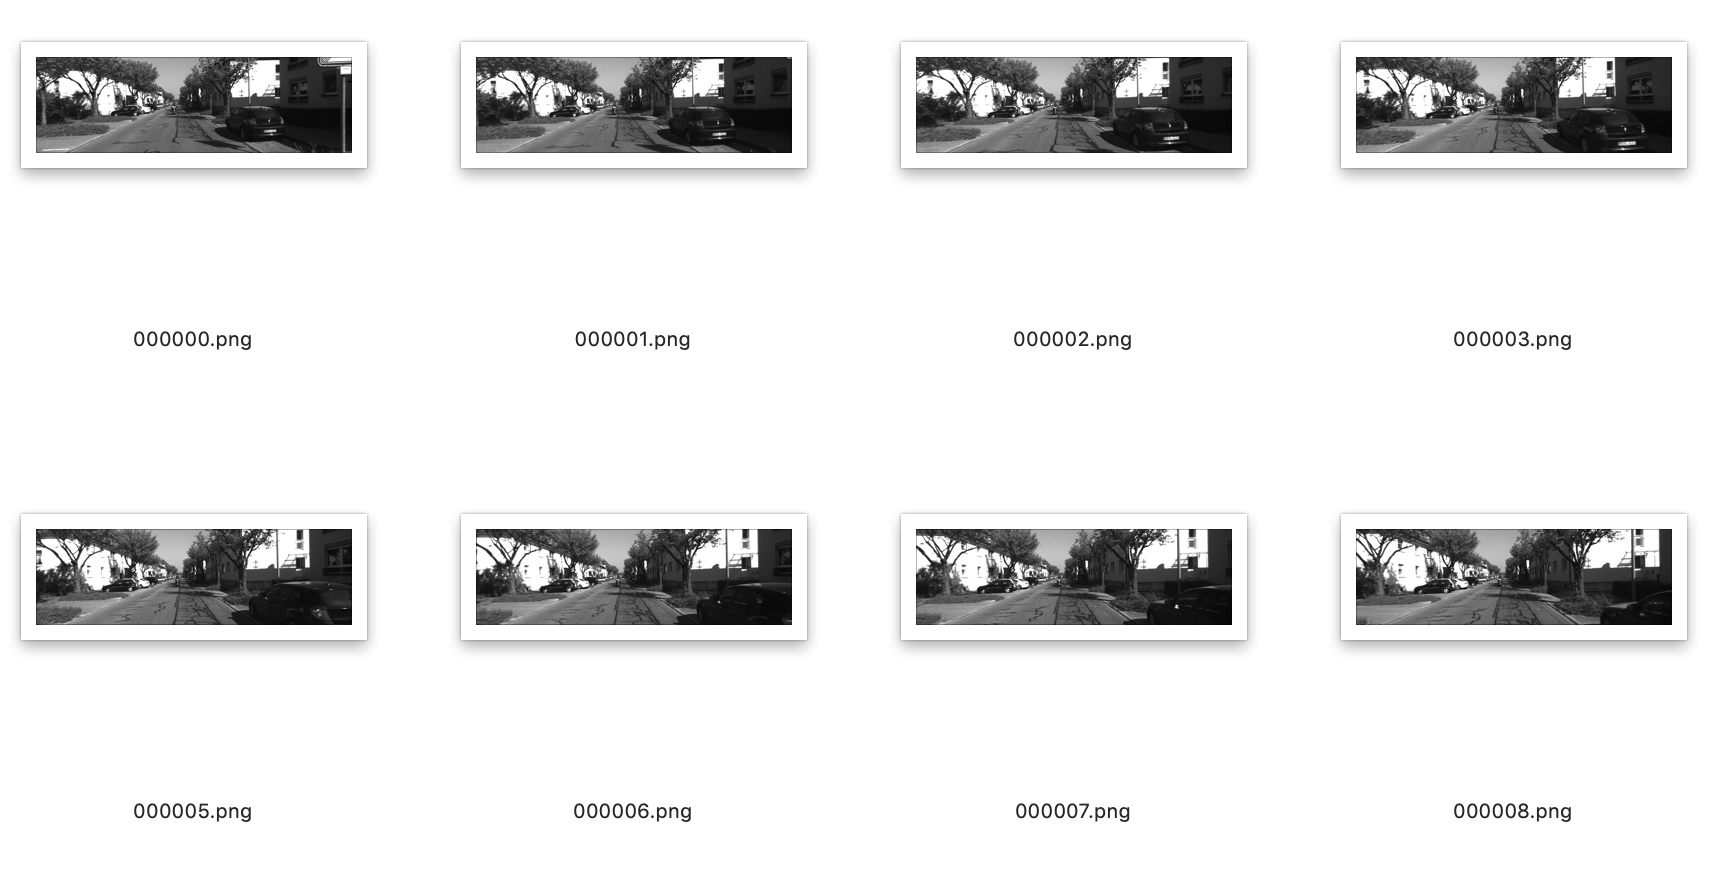
\includegraphics[width=5in]{Chapter4/kittiexamples.eps}
	\caption{Example image in KITTI Visual Odometry 2012 dataset.}
	\label{fig:kittiexamples} 
\end{figure}

\subsection{Oxford RobotCar Dataset}
Oxford RobotCar Dataset is presented by Will Maddern et al. in \cite{maddern20171}, as a challenging dataset for autonomous driving. Collected over the period of May 2014 to December 2015, this datasets recorded images from 6 cameras mounted Nissan LEAF, along with LIDAR, GPS and INS ground truth. Images were recorded under different weather and illumination condition  from 9:00 to 16:00 on average, from May to December. Example images is shown in Figure \ref{fig:robotcarexamples}.

\begin{figure}[H]
	\centering
	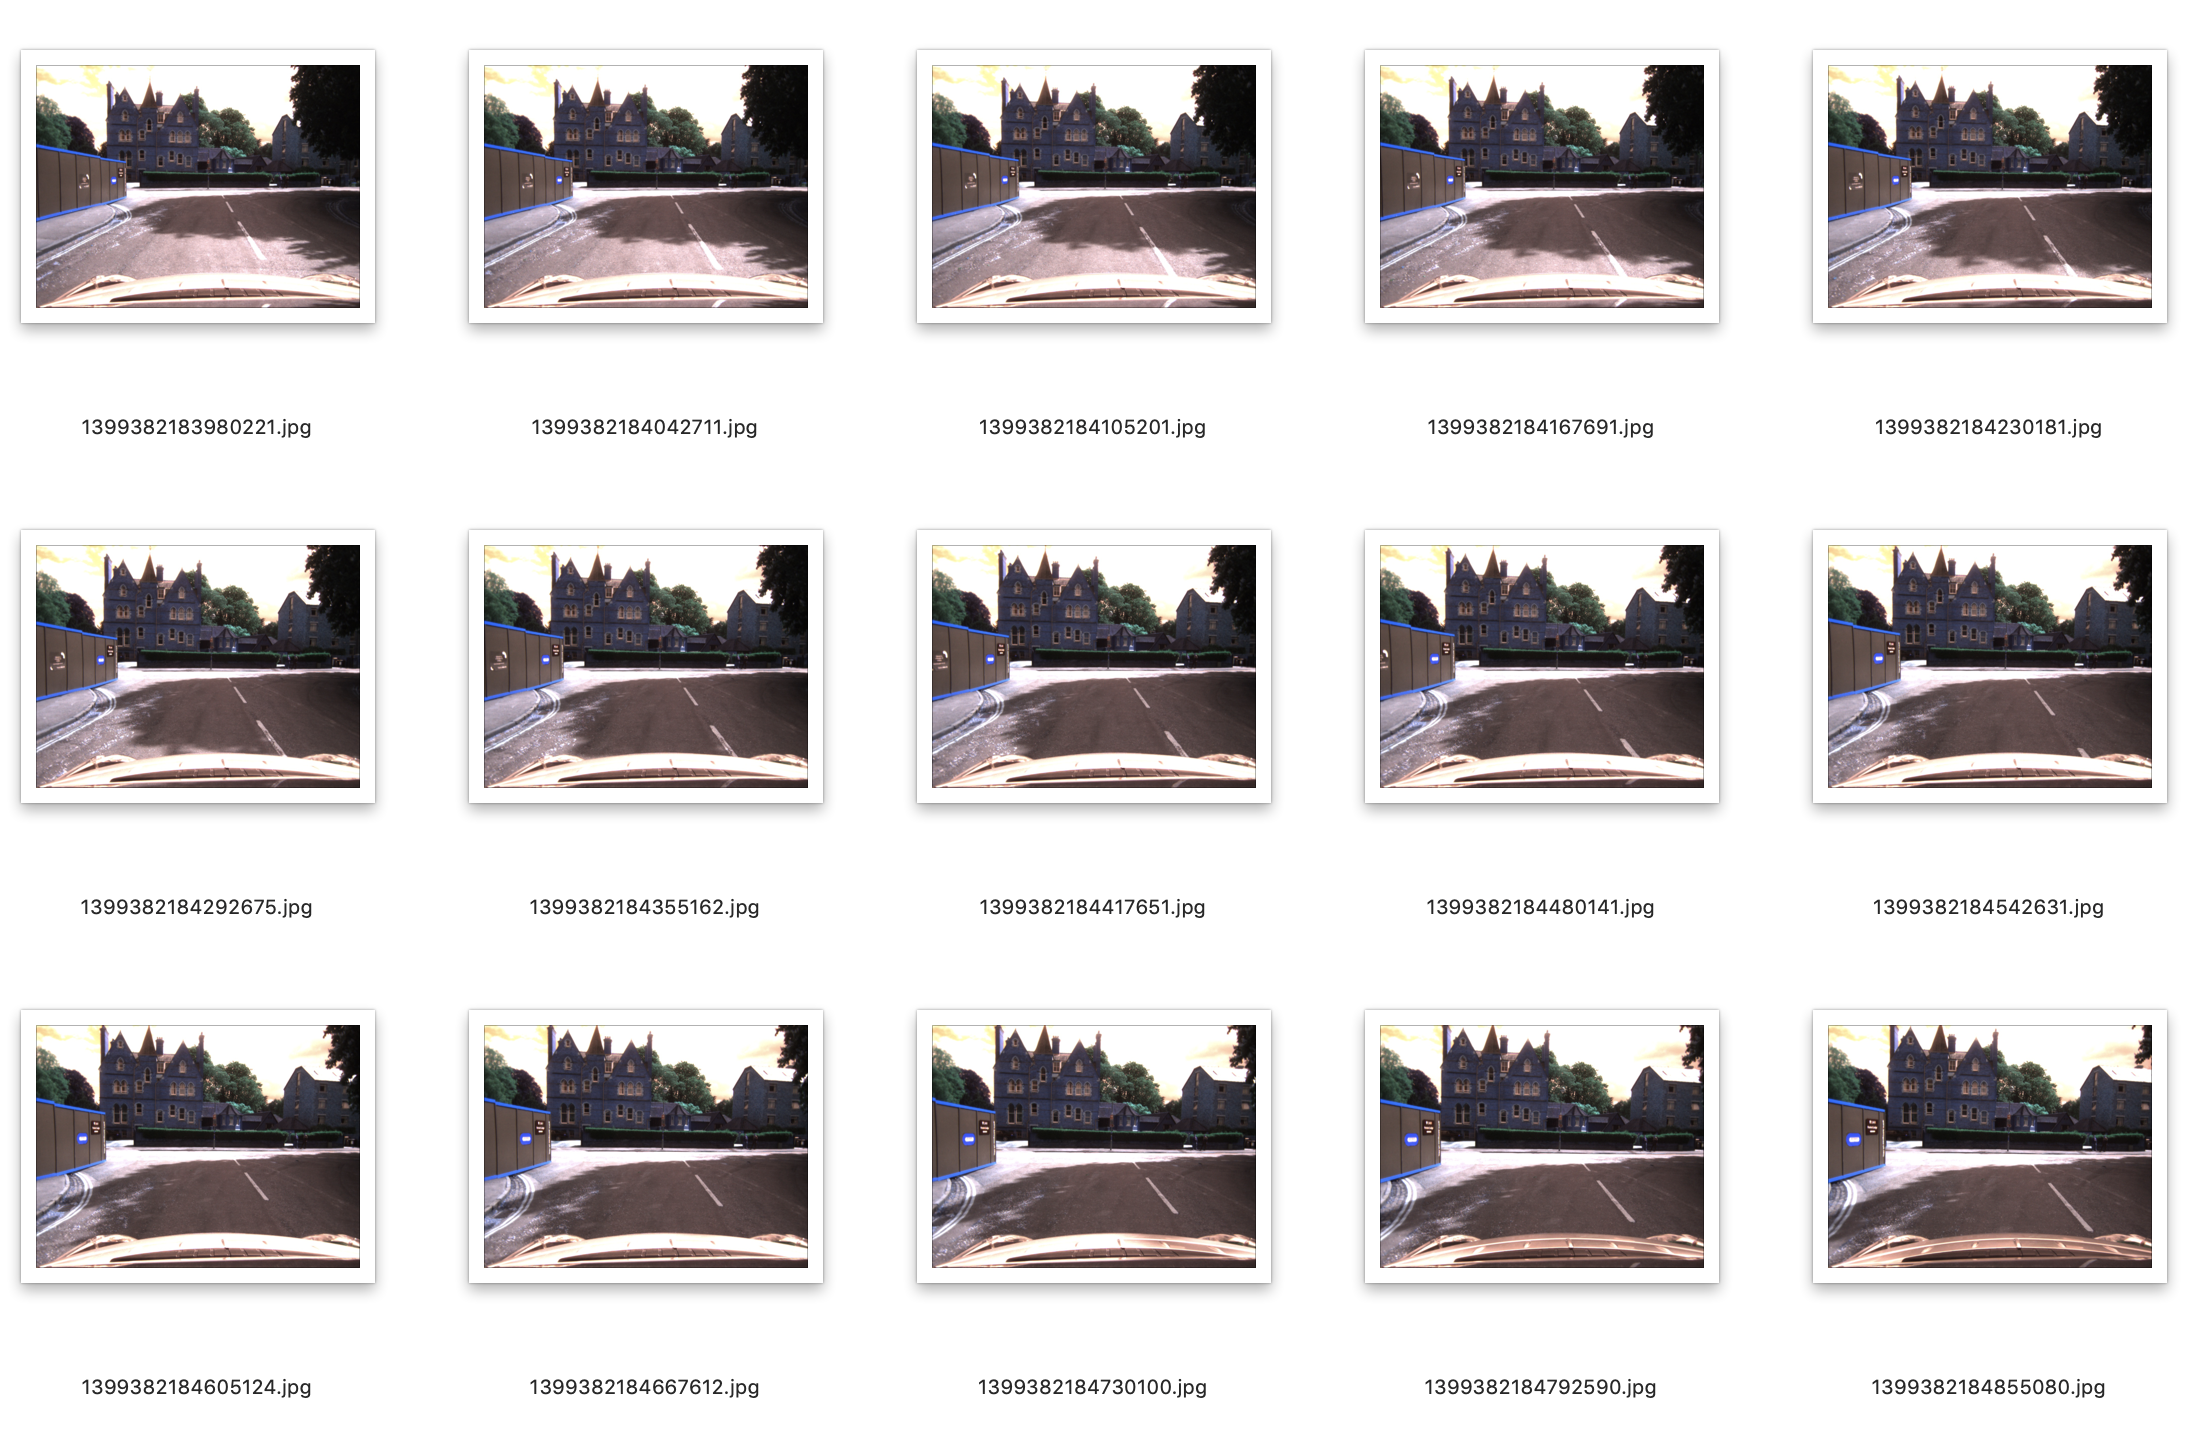
\includegraphics[width=5in]{Chapter4/robotcarexamples.eps}
	\caption{Example image in robotcar dataset.}
	\label{fig:robotcarexamples} 
\end{figure}

The RobotCar platform is a Nissan LEAF equipped with sensors as following \cite{maddern20171}:

\begin{enumerate}
	\item Stereo Camera: Bumblebee XB3 trinocular stereo camera $\times$ 1, 1/3'' Sony ICX445 CCD, 1280$\times$960$\times$3, 16Hz, 3.88mm lens, $66^{\circ}$ HFoV, 12/24cm baseline, global shutter.
	\item Monocular Camera: Grasshopper2 $\times$ 3, 2/3'' ICX285 CCD, 1024$\times$1024, 11.1Hz, 2.67mm fisheye lens, $180^{\circ}$, global shutter.
	\item 2D LIDARL SICK LMS-151 2D LIDAR $\times$ 2, $270^{\circ}$ FoV, 50Hz, 50m range, $0.5^{\circ}$ resolution.
	\item 3D LIDAR: SICK LD-MRS 3D LIDAR $\times$ 1, $85^{\circ}$ HFoC, $3.2^{\circ}$ VFoV, 4 panes, 12.5Hz, 50m range, $0.125^{\circ}$ resolution.
	\item GPS/INS Module: NovAtel SPAN-CPT ALIGN inertial and GPS navigation system $\times$ 1, 6 axis, 50Hz, GPS/GLONASS, dual antenna.
 \end{enumerate}

The RobotCar platform and the sensor locations are demonstrated in Figure \ref{fig:robotcarsensorlocation}.

\begin{figure}[H]
	\centering
	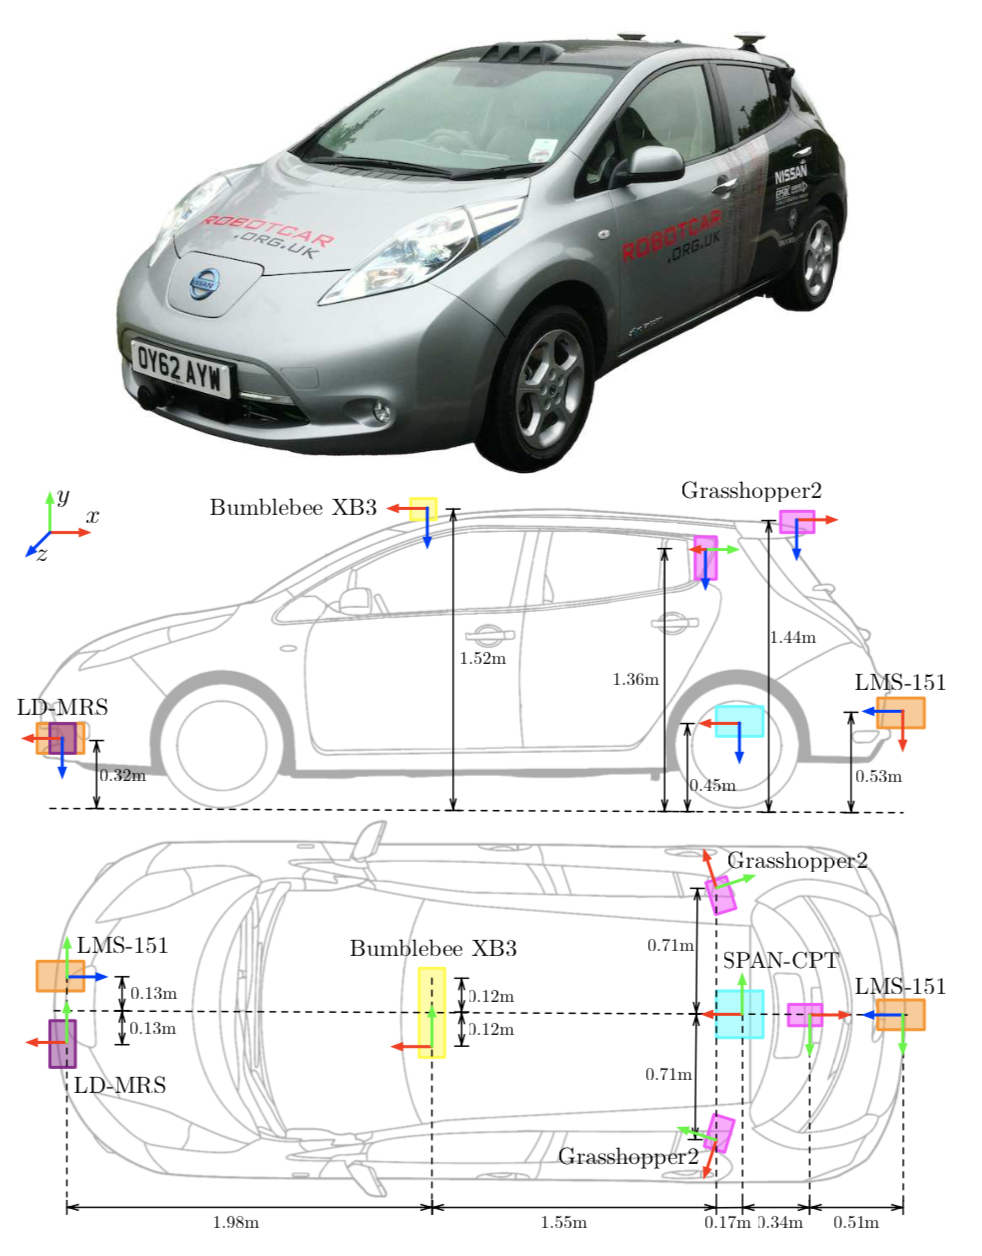
\includegraphics[width=5in]{Chapter4/robotcarsensorlocation.eps}
	\caption{The robotcar platform and sensor location diagram.}
	\label{fig:robotcarsensorlocation} 
\end{figure}

RobotCar dataset is especially suitable to evaluate long-term SLAM systems, since it contains images taken in different hours of daytime under different illumination conditions, and in different seasons. The comparison between image in different illumination conditions and different seasons is shown in Figure \ref{fig:robotcarcomparisonseason}.

\begin{figure}
	\centering
	\subfigure[Image captured in 14:49 07/14/2014.]{
		\label{sfig:robotcarjulyraw}
		\begin{minipage}[t]{0.4\linewidth}
			\centering
			\includegraphics[width=2in]{Chapter4/robotcarfeb.eps}
			%\caption{fig1}
		\end{minipage}
	}
	\subfigure[Image captured in 12:32 02/24/2015.]{
	\label{sfig:robotcarfebraw}
		\begin{minipage}[t]{0.4\linewidth}
			\centering
			\includegraphics[width=2in]{Chapter4/robotcardec.eps}
			%\caption{fig2}
		\end{minipage}
	}
	\caption{Comparison of images captured in the same location in different seasons in RobotCar dataset.}
	\label{fig:robotcarcomparisonseason}
\end{figure}
	
\subsection{NTU Dataset}
\label{sec:ntuinfo}
Our NTU dataset \cite{zhang2018two} is collected by multi ground robots consisting of two husky UGV platforms, recording driving around the carpark in front of School of EEE building.

Our UGV platform is a HUSKY Clearpath robot, equipped with a ZED stereo camera $\times$ 1, 672$\times$376, $87^{\circ}$ HFoV, $56^{\circ}$ VFoV. The picture of the platform and example images are shown in Figure \ref{fig:ntuugvplatform} and \ref{fig:ntuexamples}.

%The UAV platform is assembled with: PIXRACER V1.0 AUTOPILOT Controller Module, DJI E Series 620S Motor Package, a uBLOXNEO-M8N GPS Module and a monocular camera mounted at a depression angle of 20 degree. The overview picture of the UAV is shown in Figure \ref{fig:ntuuavplatform}

The dataset provides 4 rosbag files. 3 of them are recorded by UGV, while the other one is recorded by UAV. The basic information of 4 rosbags are listed in Table \ref{tbl:ntubagsinfo}. And the ground truth trajectories are shown in Figure \ref{fig:ntugt}.

\begin{figure}
	\centering
	\subfigure[Ground truth trajectory of Bag.0.]{
		\begin{minipage}[t]{0.4\linewidth}
			\centering
			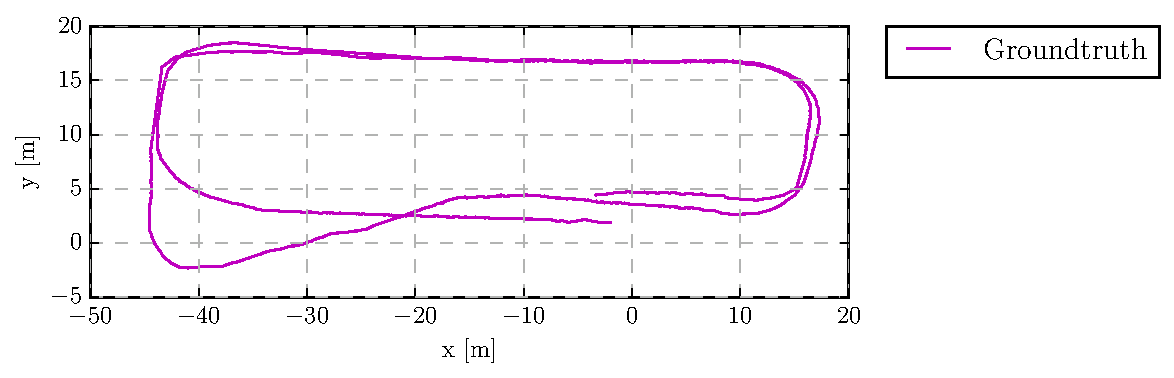
\includegraphics[width=2in]{Chapter4/NTU/0446/plots/trajectory_top_gt_sim3_-1.pdf}
			%\caption{fig1}
		\end{minipage}
	}
	\subfigure[Ground truth trajectory of Bag.1.]{
		\begin{minipage}[t]{0.4\linewidth}
			\centering
			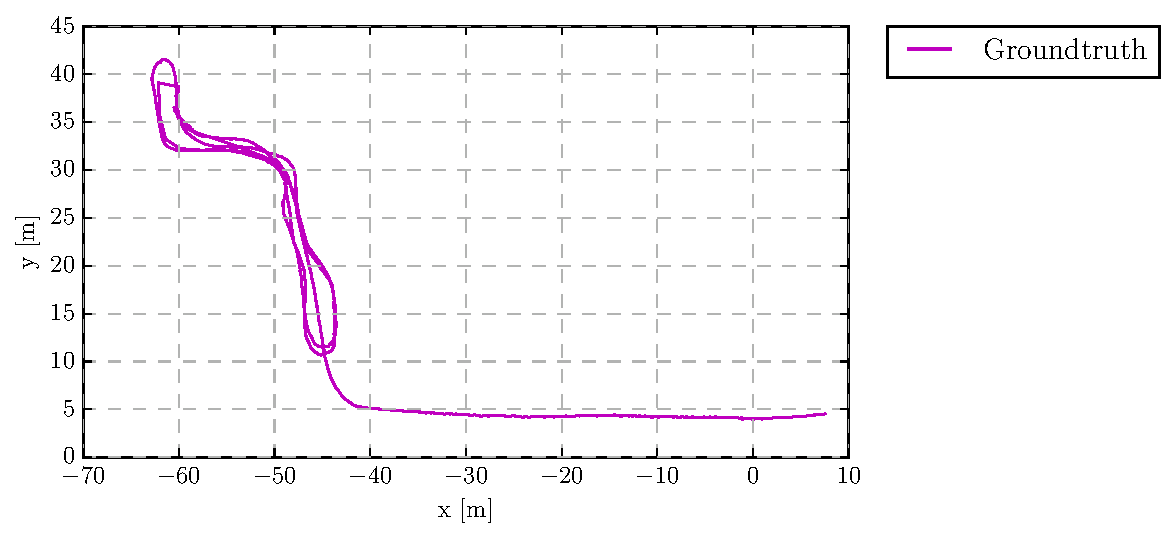
\includegraphics[width=2in]{Chapter4/NTU/0454/plots/trajectory_top_gt_sim3_-1.pdf}
			%\caption{fig2}
		\end{minipage}
	}
%	\vfill
%		\subfigure[Ground truth trajectory of Bag.2.]{
%		\begin{minipage}[t]{0.4\linewidth}
%			\centering
%			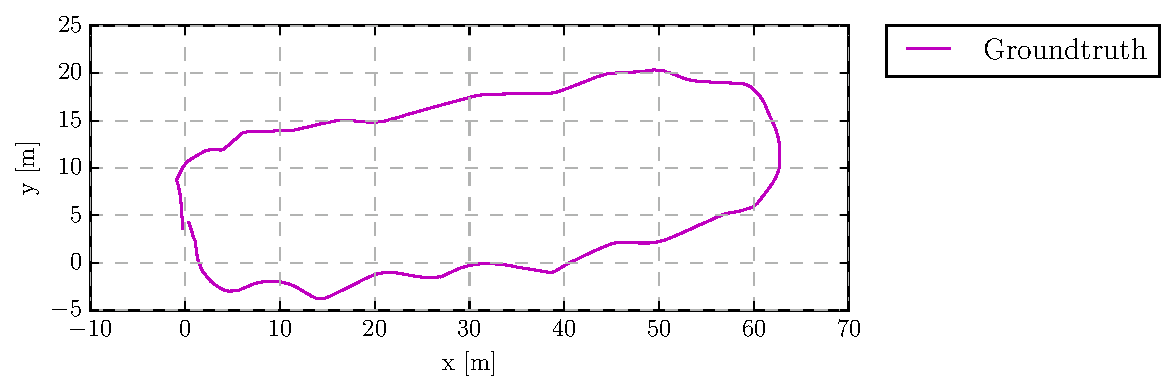
\includegraphics[width=2in]{Chapter4/NTU/UGV/plots/trajectory_top_gt_sim3_-1.pdf}
%			%\caption{fig1}
%		\end{minipage}
%	}
%	\subfigure[Ground truth trajectory of Bag.3.]{
%		\begin{minipage}[t]{0.4\linewidth}
%			\centering
%			
\includegraphics[width=2in]{thereisafigure.eps}
%			%\caption{fig2}
%		\end{minipage}
%	}
	\caption{Ground truth information of each rosbags in NTU Dataset.}
	\label{fig:ntugt}
\end{figure}

\begin{table*}
	\centering
	\caption{Main characteristics of the rosbags in NTU Dataset used in the experiment.}
	\begin{tabular}{|c|c|c|c|c|}
		\hline
		Bag No. & Data(M/D/Y)  & Platform & Height(m) & Dep. Angle  \\
		\hline
		0&10/27/2018& UGV & $\approx 0.7m$ & $0^\circ$ \\
		\hline
		1&10/27/2018& UGV & $\approx 0.7m$ & $0^\circ$ \\
		\hline
%		2&03/08/2019& UGV & $\approx 0.7m$ & $0^\circ$ \\
%		\hline
%		3&03/08/2019& UAV & $\approx 2m$ & $20^\circ$ \\
%		\hline
	\end{tabular}
	\label{tbl:ntubagsinfo}
\end{table*}

\begin{figure}[H]
	\centering
	\includegraphics[width=5in]{Chapter4/ntuhuskytugv.eps}
	\caption{Overview picture of NTU Husky platform.}
	\label{fig:ntuugvplatform} 
\end{figure}

%\begin{figure}[H]
%	\centering
%	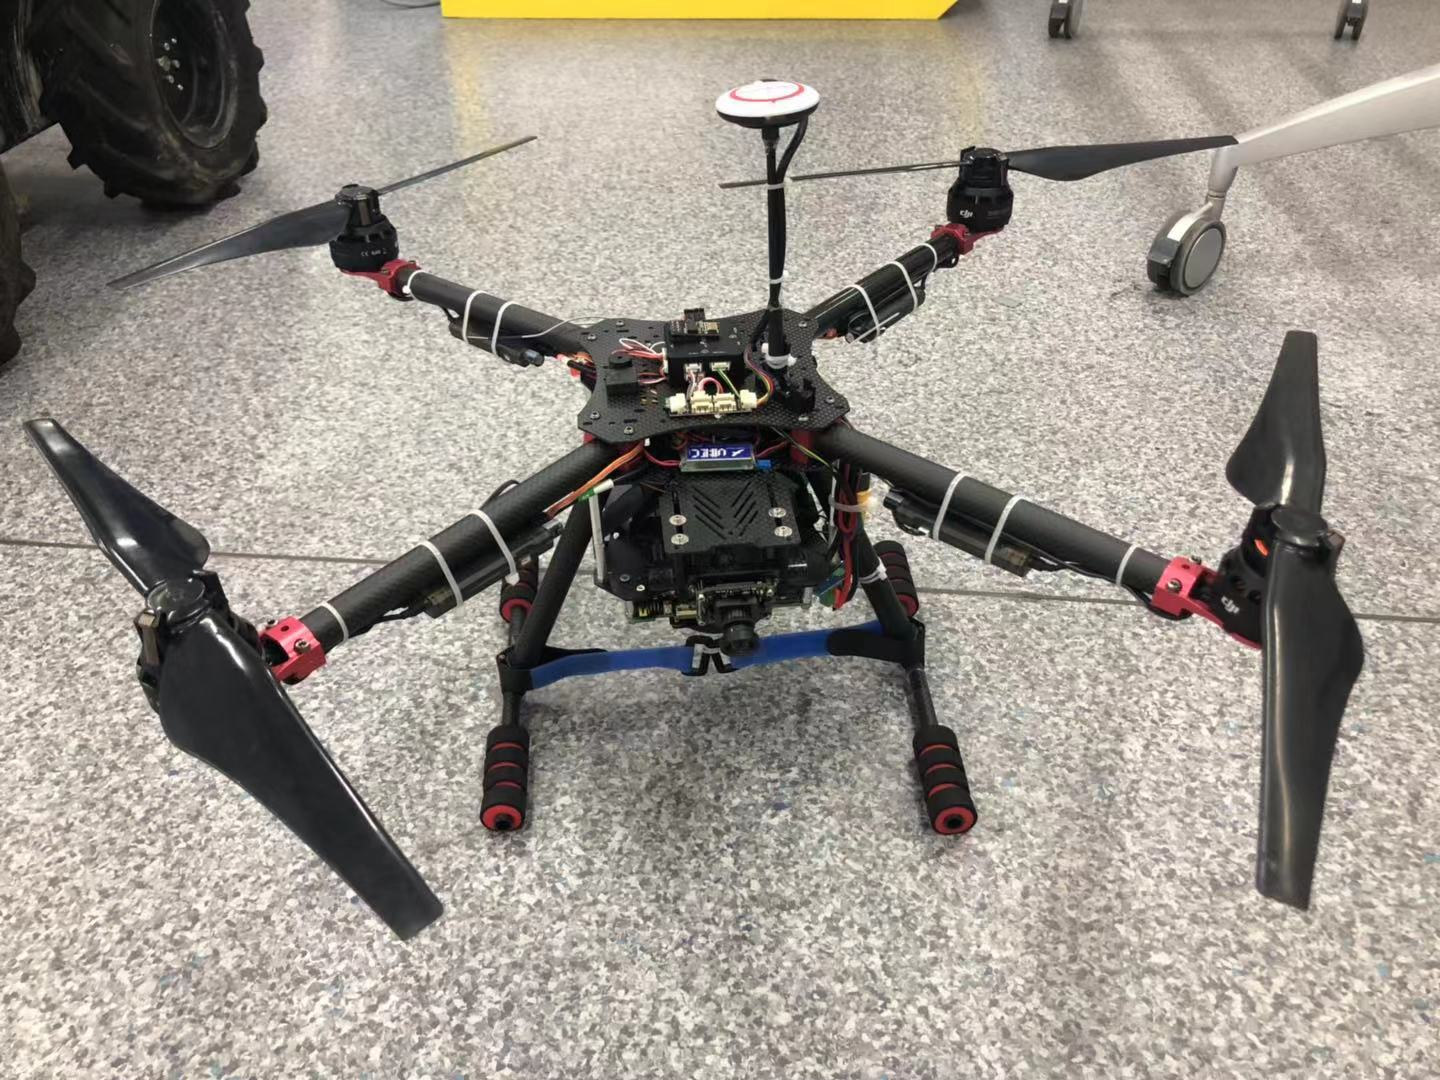
\includegraphics[width=5in]{Chapter4/ntuuav0.eps}
%	\caption{Overview picture of NTU Husky platform.}
%	\label{fig:ntuuavplatform} 
%\end{figure}

\begin{figure}[H]
	\centering
	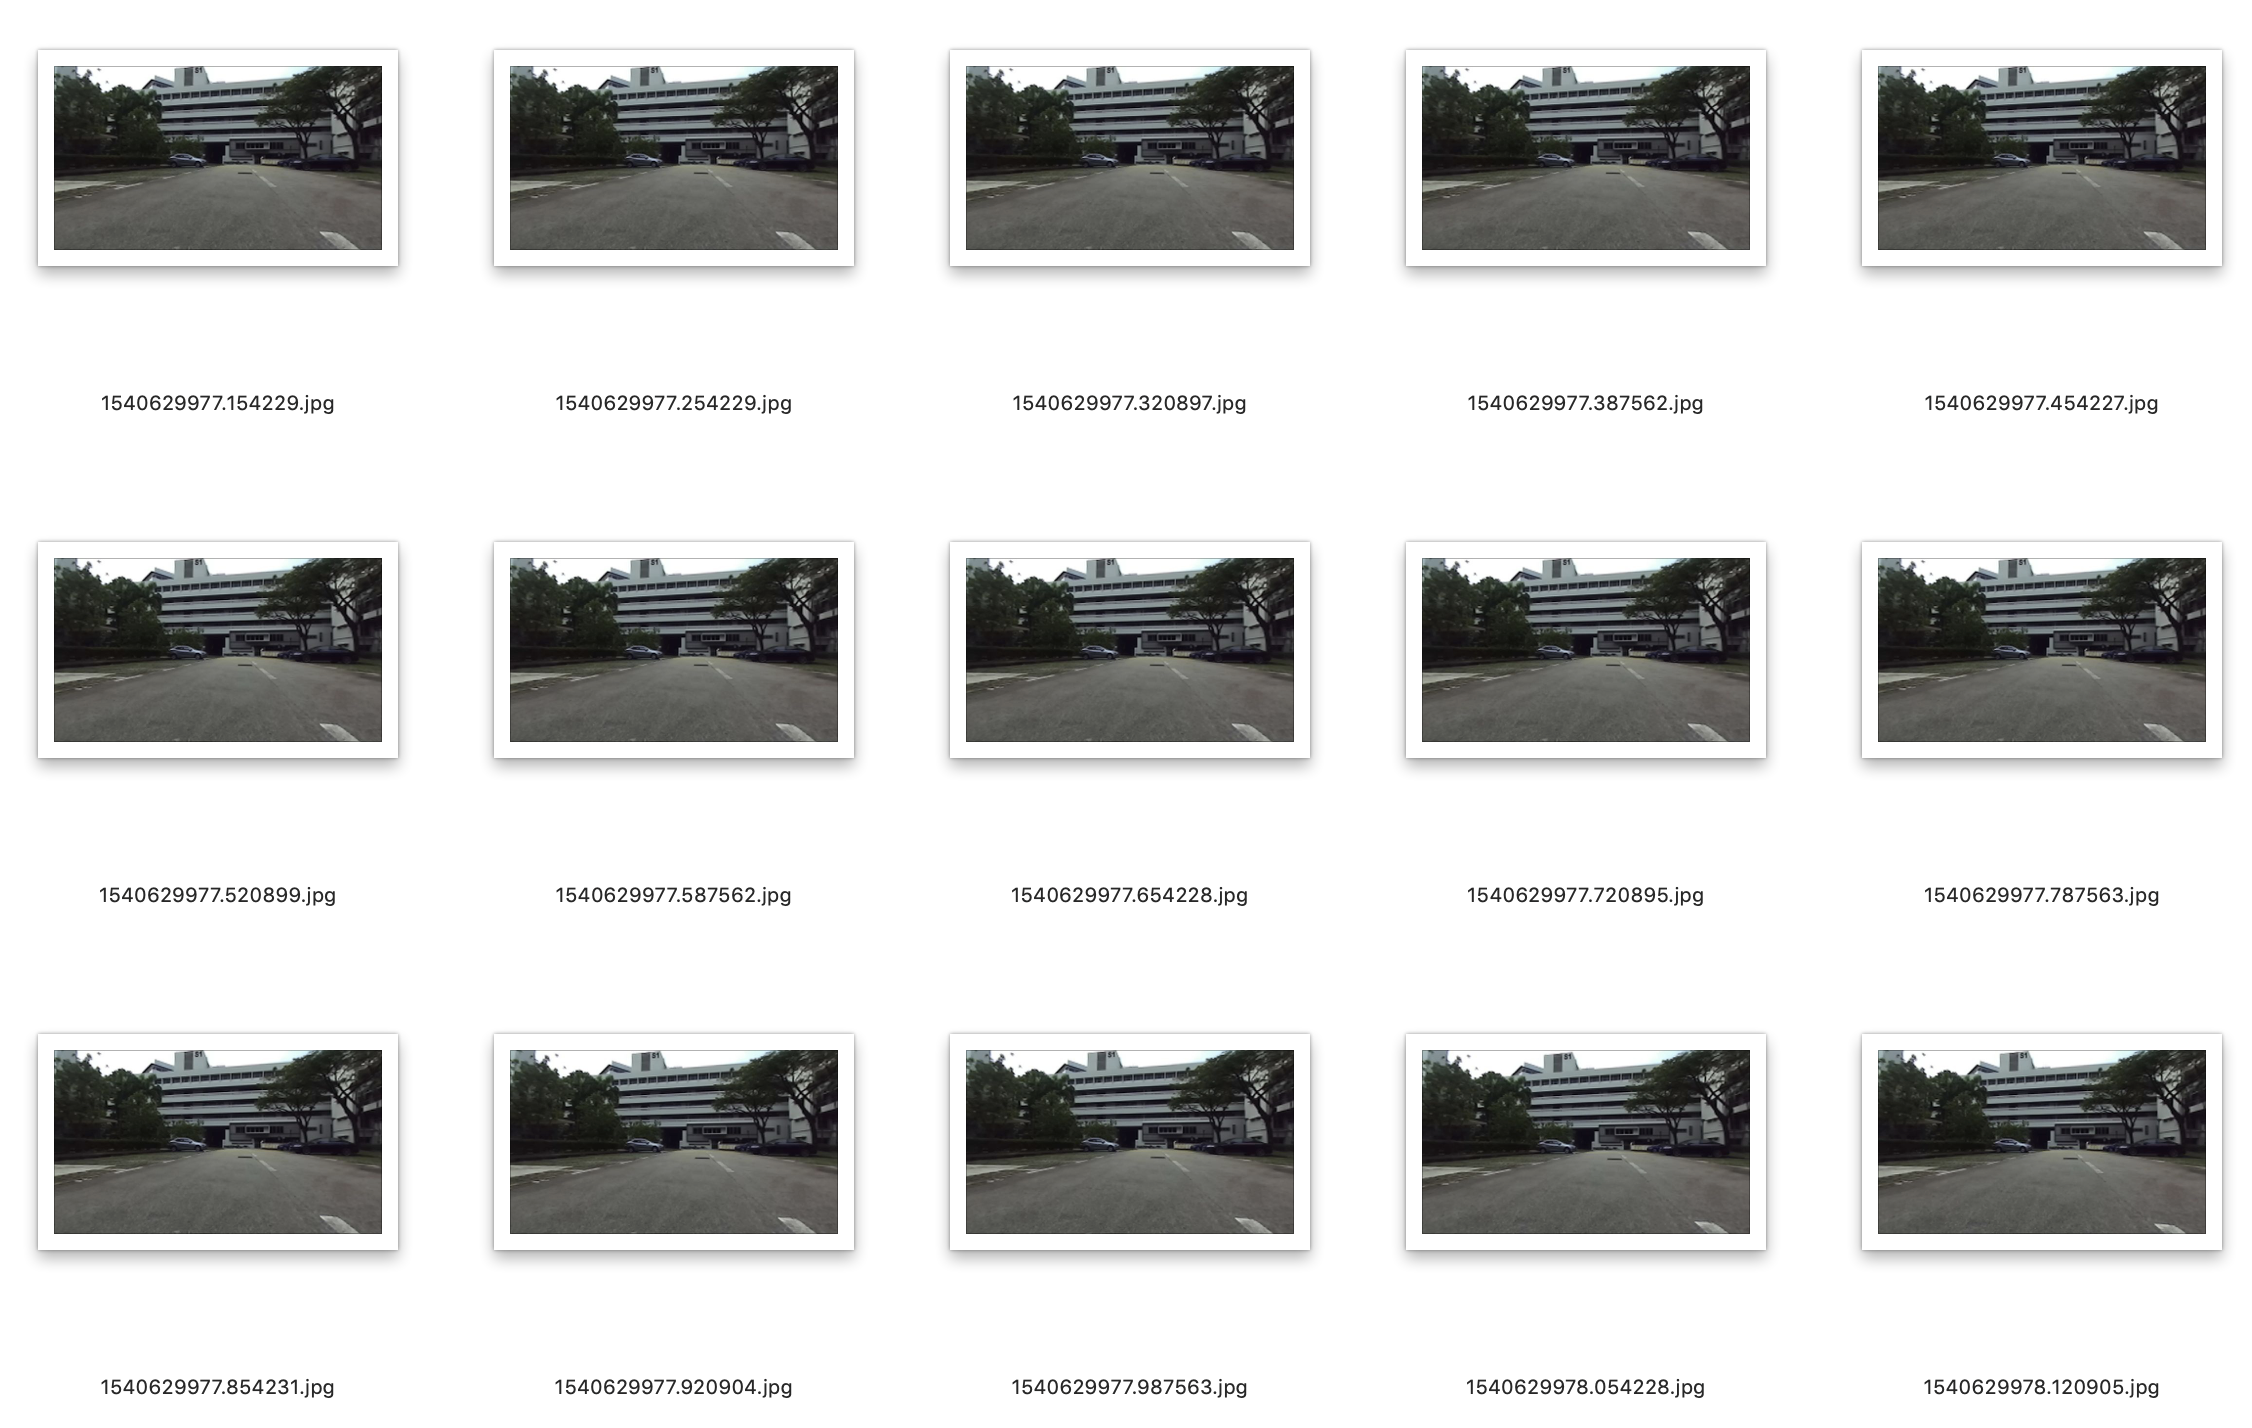
\includegraphics[width=5in]{Chapter4/ntuexamples.eps}
	\caption{Example images of NTU dataset.}
	\label{fig:ntuexamples} 
\end{figure}

\section{Evaluation of CORBSLAM}

\ifoutputscaleerror
\subsection{Evaluation on multi ground robots}
\fi

\subsection{KITTI Datasets}
\label{sec:kittievaluate}
In order to evaluate CORB-SLAM system, sequence 00 is utilized and separated into two sub sequences with proper length of overlap. The following separating method is employed: We assume the time period of a KITTI sequence if $Seq.0[0,t]$. Then the sequence is separated into two sub sequences $Seq.01[0,\frac{t}{2}+\delta{t}]$ and $Seq.02[\frac{t}{2},t]$ as the assumed input of two client robots. 

Therefore, in this case, Sequence 00 containing $f=4541frames$ and covering a total distance of $s=1856m$ is separated into two partial sequences: Seq.0$[0, \frac{2}{3}f]$ and Seq.1$[\frac{1}{3}f, f]$, both containing  $\frac{2}{3}f\approx{3027frames}$ and covering distances of $\frac{2}{3}s\approx{1237m}$ (a rough estimate since distances between each pair of frames are not equal). 

The ground truth information of Seq.0, Seq.1 and the complete ground truth trajectory of Sequence 00 are shown for reference in Figure \ref{fig:kittigt}. And Figure \ref{fig:kittiresults} demonstrates mapping results of each partial sequence and the map fusion results of the server. Four charts in Figure \ref{fig:kittiquanresult} contains quantitative evaluation results, with corresponding numeric results shown in Table \ref{tbl:ntuquanresult}.

Clients' quantitative mapping results of each partial sequence are provided in Figure \ref{fig:kittiseq0quanresult}, \ref{fig:kittiseq1quanresult}  and Table \ref{tbl:kittiseq0quanresult}, \ref{tbl:kittiseq1quanresult}. And because the two partial sequences are extracted from Sequence 00, so the completed mapping results of CORB-SLAM client on Sequence 00 can be provided as a comparison by Figure \ref{fig:kittientirequanresult}, \ref{fig:kitticlientmapping} and Table \ref{tbl:kitticlientquanresult} in the same format as above. Results are further discussed in Section \ref{sec:disussmultiground}.


\begin{figure}
	\centering
	\subfigure[Ground truth trajectory of Seq.0.]{
		\begin{minipage}[t]{0.4\linewidth}
			\centering
			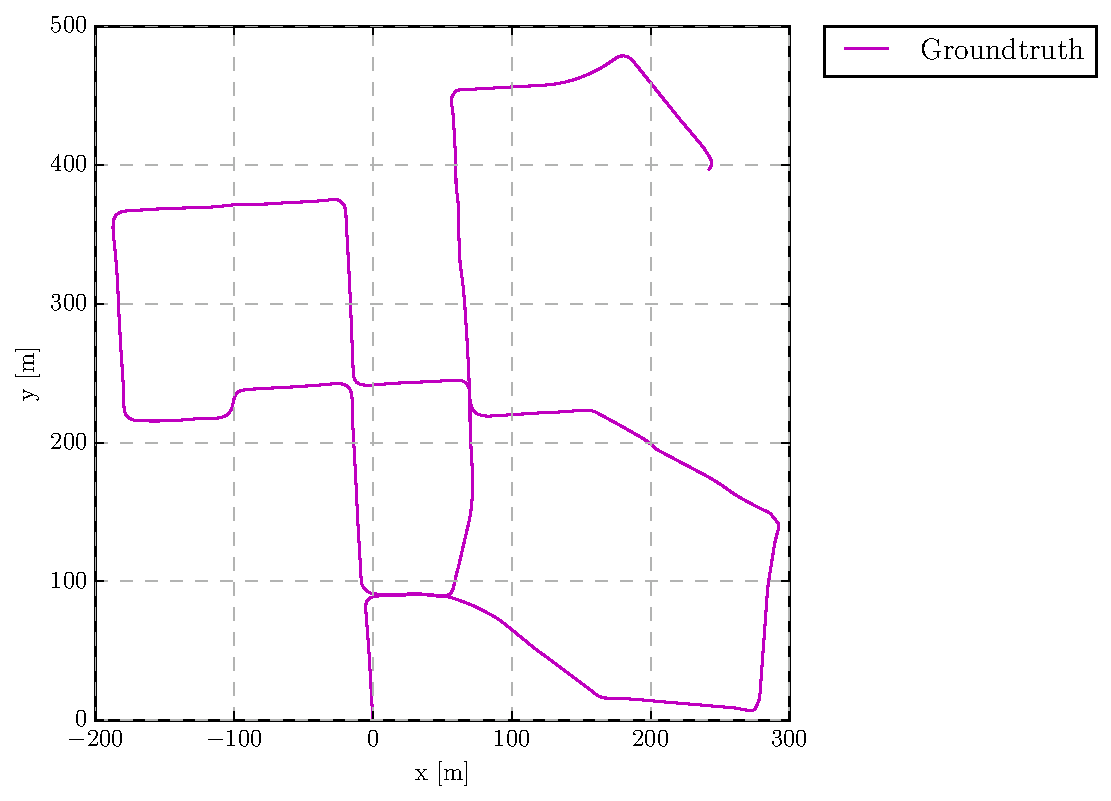
\includegraphics[width=2in]{Chapter4/KITTI/00server/32/plots/trajectory_side_gt_sim3_-1.pdf}
			%\caption{fig1}
		\end{minipage}
	}
	\subfigure[Ground truth trajectory of Seq.1.]{
		\begin{minipage}[t]{0.4\linewidth}
			\centering
			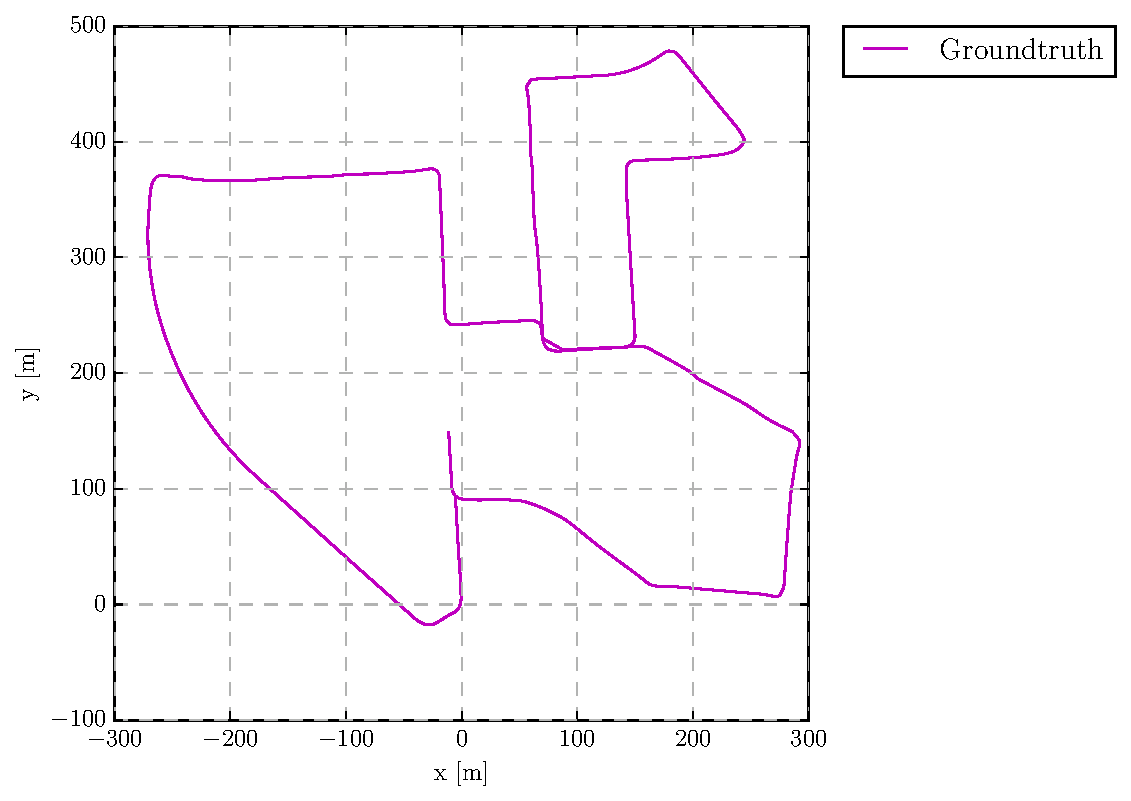
\includegraphics[width=2in]{Chapter4/KITTI/00server/33/plots/trajectory_side_gt_sim3_-1.pdf}
			%\caption{fig2}
		\end{minipage}
	}
	\vfill
	\subfigure[Ground truth trajectory of complete Sequence 00.]{
		\begin{minipage}[t]{\linewidth}
			\centering
			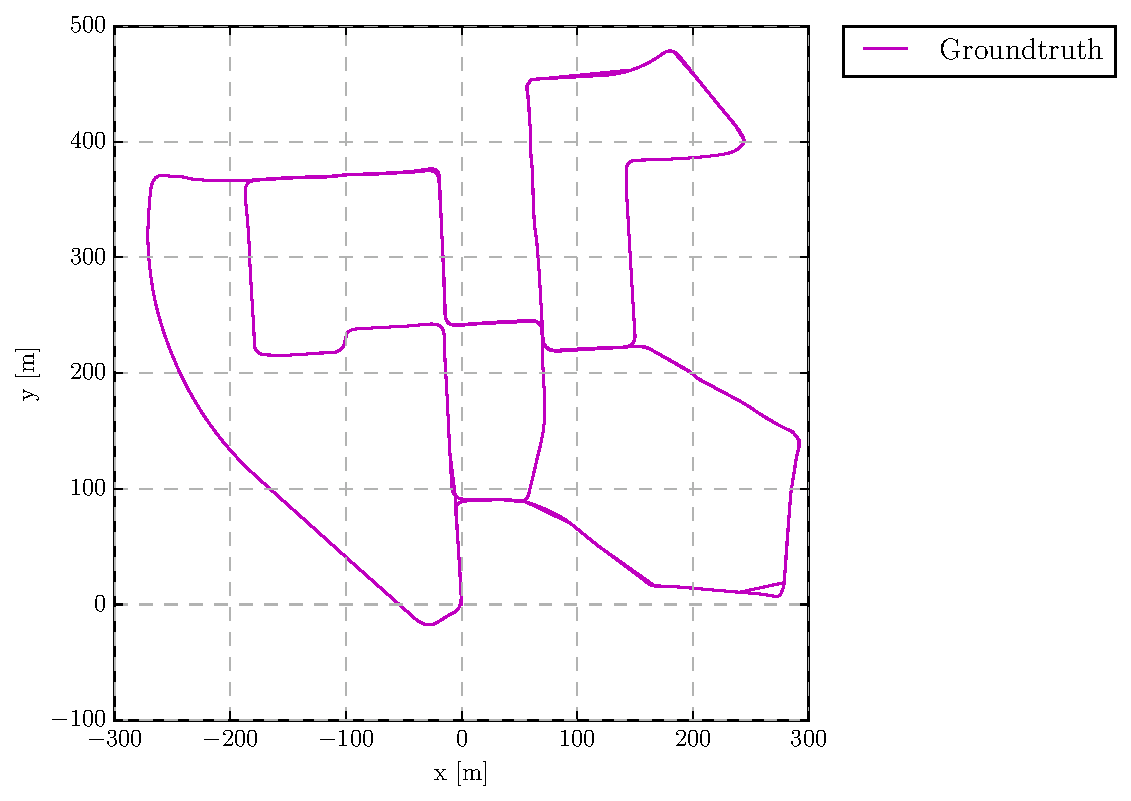
\includegraphics[width=5in]{Chapter4/KITTI/00server/plots/trajectory_side_gt_sim3_-1.pdf}
			%\caption{fig1}
		\end{minipage}
	}
	\caption{Ground truth trajectory of partial and complete sequences of KITTI Datasets.}
	\label{fig:kittigt}
\end{figure}

\begin{figure}
	\centering
	\subfigure[Relative translation error.]{
		\begin{minipage}[t]{0.4\linewidth}
			\centering
			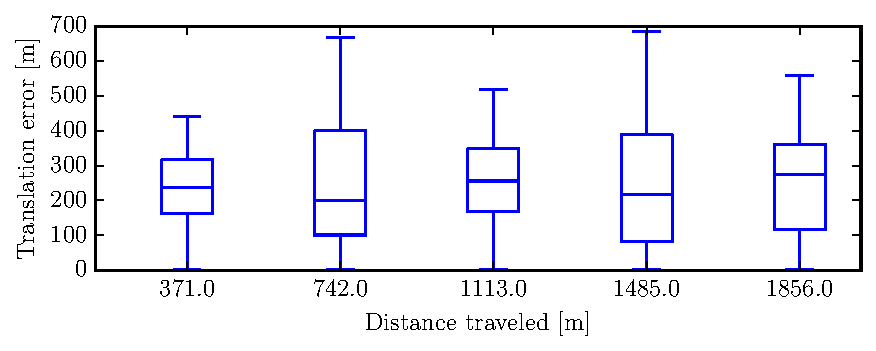
\includegraphics[width=2in]{Chapter4/KITTI/00/gps/plots/rel_translation_error.pdf}
			%\caption{fig1}
		\end{minipage}
	}
	\subfigure[Relative translation error by percent.]{
		\begin{minipage}[t]{0.4\linewidth}
			\centering
			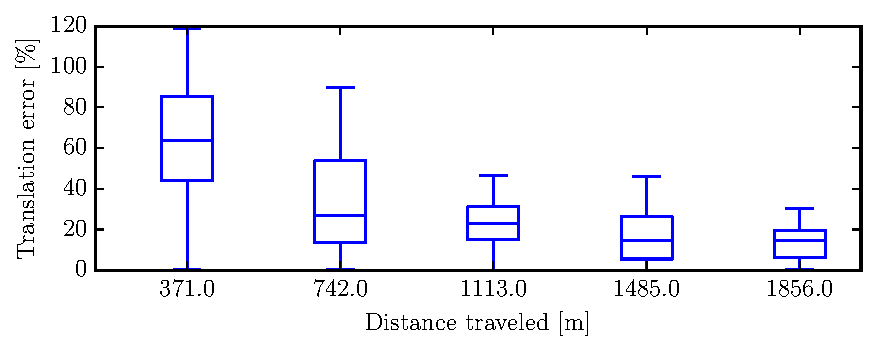
\includegraphics[width=2in]{Chapter4/KITTI/00/gps/plots/rel_translation_error_perc.pdf}
			%\caption{fig2}
		\end{minipage}
	}
	\vfill
	\subfigure[Relative yaw error.]{
		\begin{minipage}[t]{0.4\linewidth}
			\centering
			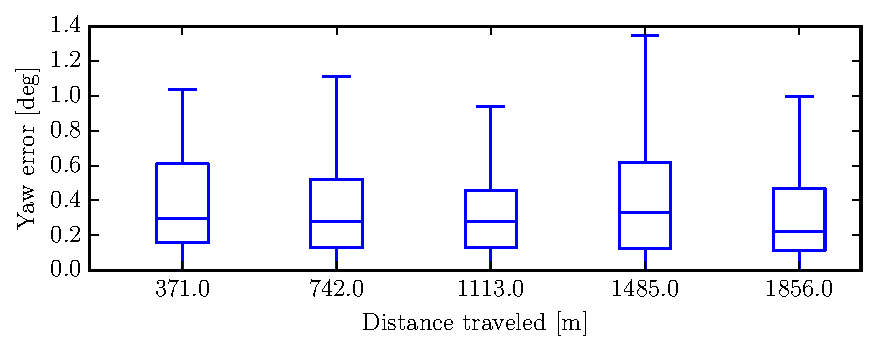
\includegraphics[width=2in]{Chapter4/KITTI/00/gps/plots/rel_yaw_error.pdf}
			%\caption{fig1}
		\end{minipage}
	}
\ifoutputscaleerror
	\subfigure[Scale error.]{
		\begin{minipage}[t]{0.4\linewidth}
			\centering
			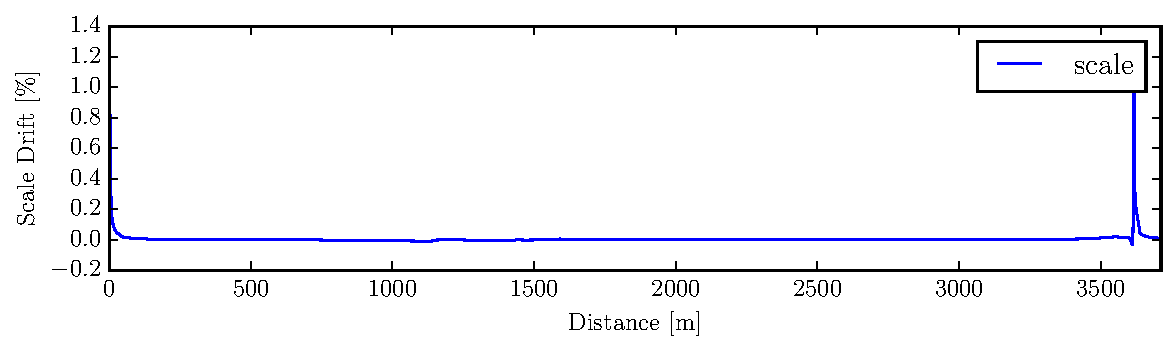
\includegraphics[width=2in]{Chapter4/KITTI/00/gps/plots/scale_error_sim3_-1.pdf}
			%\caption{fig2}
		\end{minipage}
	}
\fi
	\caption{Quantitative evaluation results of CORB-SLAM client mapping the entire KITTI Sequence 00.}
	\label{fig:kittientirequanresult}
\end{figure}

\begin{figure}
	\centering
	\subfigure[Relative translation error.]{
		\begin{minipage}[t]{0.4\linewidth}
			\centering
			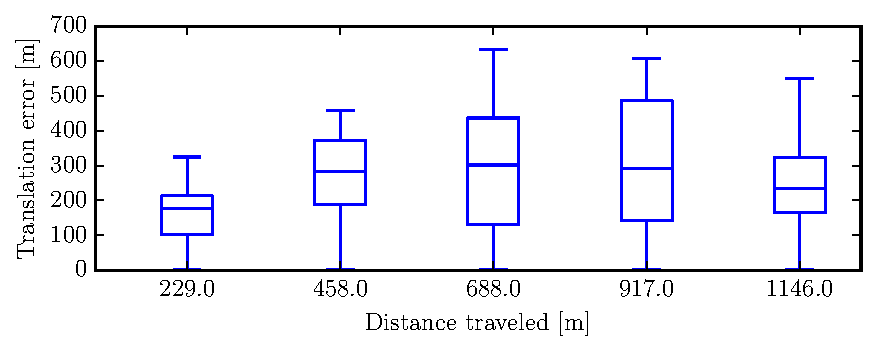
\includegraphics[width=2in]{Chapter4/KITTI/00server/32/plots/rel_translation_error.pdf}
			%\caption{fig1}
		\end{minipage}
	}
	\subfigure[Relative translation error by percent.]{
		\begin{minipage}[t]{0.4\linewidth}
			\centering
			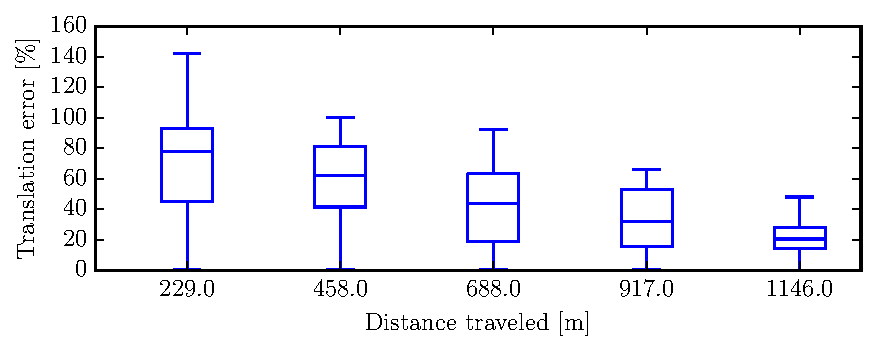
\includegraphics[width=2in]{Chapter4/KITTI/00server/32/plots/rel_translation_error_perc.pdf}
			%\caption{fig2}
		\end{minipage}
	}
	\vfill
	\subfigure[Relative yaw error.]{
		\begin{minipage}[t]{0.4\linewidth}
			\centering
			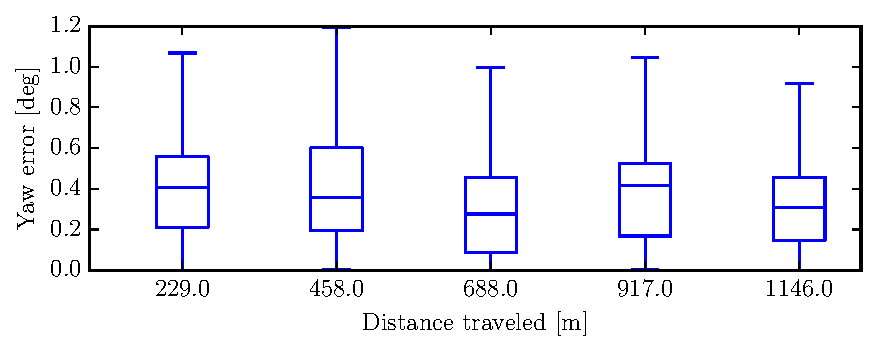
\includegraphics[width=2in]{Chapter4/KITTI/00server/32/plots/rel_yaw_error.pdf}
			%\caption{fig1}
		\end{minipage}
	}
\ifoutputscaleerror
	\subfigure[Scale error.]{
		\begin{minipage}[t]{0.4\linewidth}
			\centering
			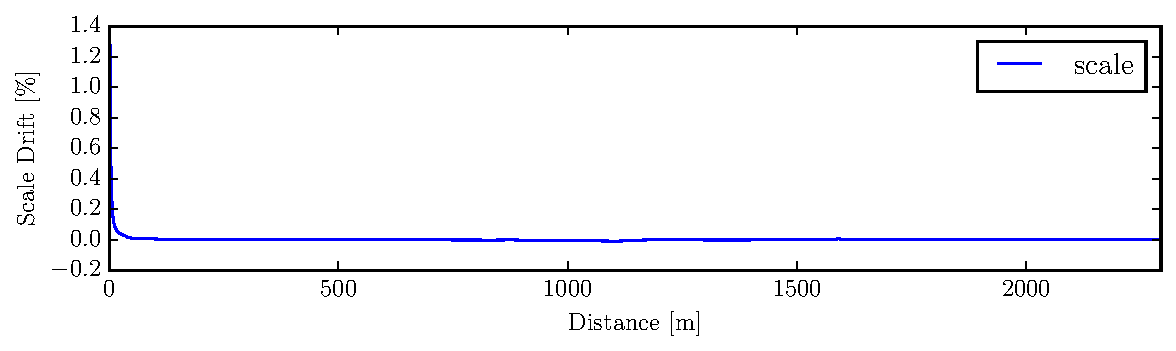
\includegraphics[width=2in]{Chapter4/KITTI/00server/32/plots/scale_error_sim3_-1.pdf}
			%\caption{fig2}
		\end{minipage}
	}
\fi
	\caption{Quantitative evaluation results of CORB-SLAM client mapping  KITTI partial Seq.0.}
	\label{fig:kittiseq0quanresult}
\end{figure}

\begin{figure}
	\centering
	\subfigure[Relative translation error.]{
		\begin{minipage}[t]{0.4\linewidth}
			\centering
			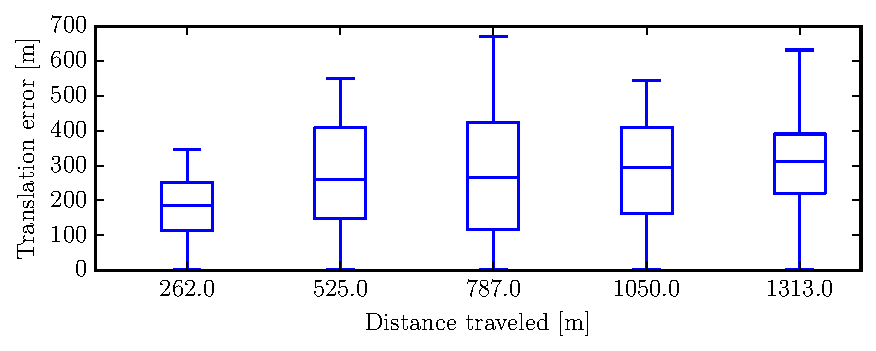
\includegraphics[width=2in]{Chapter4/KITTI/00server/33/plots/rel_translation_error.pdf}
			%\caption{fig1}
		\end{minipage}
	}
	\subfigure[Relative translation error by percent.]{
		\begin{minipage}[t]{0.4\linewidth}
			\centering
			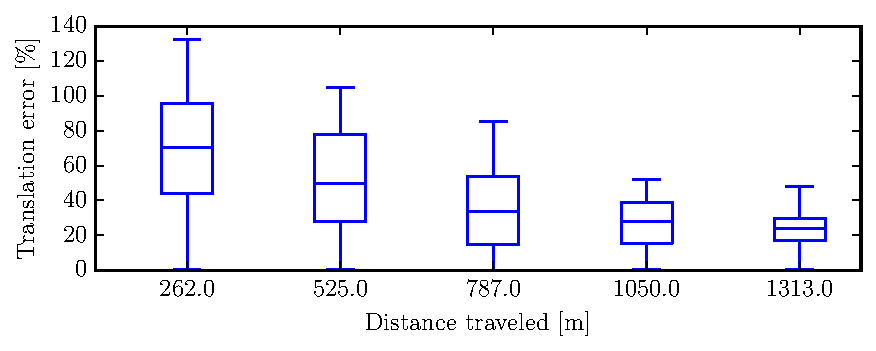
\includegraphics[width=2in]{Chapter4/KITTI/00server/33/plots/rel_translation_error_perc.pdf}
			%\caption{fig2}
		\end{minipage}
	}
	\vfill
	\subfigure[Relative yaw error.]{
		\begin{minipage}[t]{0.4\linewidth}
			\centering
			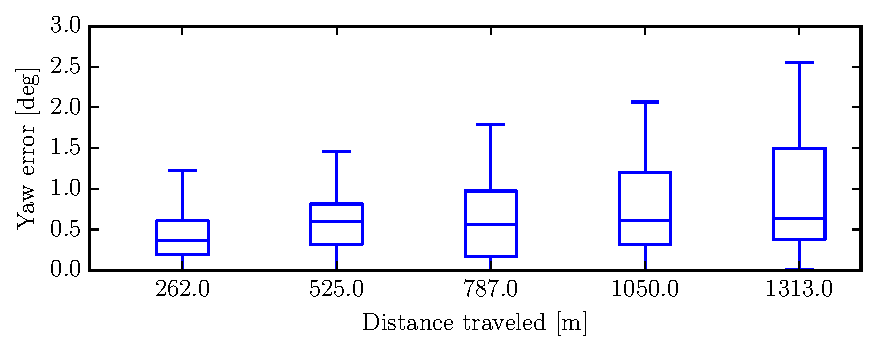
\includegraphics[width=2in]{Chapter4/KITTI/00server/33/plots/rel_yaw_error.pdf}
			%\caption{fig1}
		\end{minipage}
	}
\ifoutputscaleerror
	\subfigure[Scale error.]{
		\begin{minipage}[t]{0.4\linewidth}
			\centering
			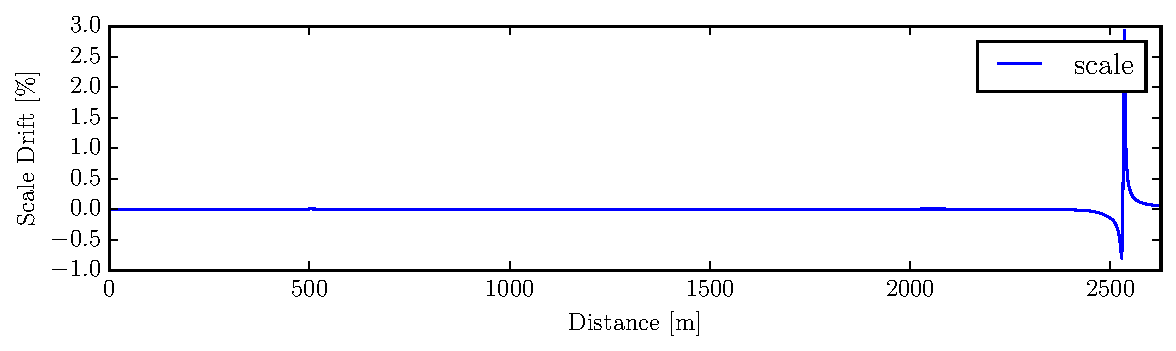
\includegraphics[width=2in]{Chapter4/KITTI/00server/33/plots/scale_error_sim3_-1.pdf}
			%\caption{fig2}
		\end{minipage}
	}
\fi
	\caption{Quantitative evaluation results of CORB-SLAM client mapping  KITTI partial Seq.1.}
	\label{fig:kittiseq1quanresult}
\end{figure}

\begin{table*}
	\centering
	\caption{Quantitative results of mapping unseparated Sequence 00.}
	\begin{threeparttable}
			\ifoutputscaleerror
		\begin{tabular}{|c|c|c|c|c|}
			\hline
			Distance(m)\tnote{1} & Rel. Trans.(m)\tnote{2}  & Rel. Trans.($\%$)\tnote{3} & Rel. Yaw(deg)\tnote{4} & Scale Err.($\%$)\tnote{5}  \\
			\hline
			371& 229.69 & 61.91 & 0.37 & - \\
			\hline
			742&260.10& 35.05 & 0.37 & - \\
			\hline
			1113&260.20& 23.38 & 0.31 & - \\
			\hline
			1485&240.93& 16.22 & 0.40 & - \\
			\hline
			1856&255.16& 13.74 & 0.32 & 0.05\\
			\hline
		\end{tabular}
		\begin{tablenotes}
			\footnotesize
			\item[1] Distance in meter traveled before each time of statistics. 
			\item[2] Mean relative translation error in meter.
			\item[3] Mean relative translation error in percent.
			\item[4] Mean relative yaw error in degree.
			\item[5] Median scale error in percent.
		\end{tablenotes}
	\fi
	
			\begin{tabular}{|c|c|c|c|c|}
		\hline
		Distance(m)\tnote{1} & Rel. Trans.(m)\tnote{2}  & Rel. Trans.($\%$)\tnote{3} & Rel. Yaw(deg)\tnote{4}   \\
		\hline
		371& 229.69 & 61.91 & 0.37  \\
		\hline
		742&260.10& 35.05 & 0.37 \\
		\hline
		1113&260.20& 23.38 & 0.31  \\
		\hline
		1485&240.93& 16.22 & 0.40 \\
		\hline
		1856&255.16& 13.74 & 0.32 \\
		\hline
	\end{tabular}
	\begin{tablenotes}
		\footnotesize
		\item[1] Distance in meter traveled before each time of statistics. 
		\item[2] Mean relative translation error in meter.
		\item[3] Mean relative translation error in percent.
		\item[4] Mean relative yaw error in degree.
	\end{tablenotes}
	\end{threeparttable}
	\label{tbl:kitticlientquanresult}
\end{table*}

\begin{table*}
	\centering
	\caption{Quantitative results of mapping Seq.0.}
	\begin{threeparttable}
		\begin{tabular}{|c|c|c|c|c|}
			\hline
			Distance(m)\tnote{1} & Rel. Trans.(m)\tnote{2}  & Rel. Trans.($\%$)\tnote{3} & Rel. Yaw(deg)\tnote{4}   \\
			\hline
			229& 161.01 & 70.31 & 0.40  \\
			\hline
			458&267.43& 58.38 & 0.42\\
			\hline
			688&299.07& 43.47 & 0.31 \\
			\hline
			917&306.37& 33.41 & 0.39 \\
			\hline
			1146&256.09& 22.35 & 0.34 \\
			\hline
		\end{tabular}
		\begin{tablenotes}
			\footnotesize
			\item[1] Distance in meter traveled before each time of statistics. 
			\item[2] Mean relative translation error in meter.
			\item[3] Mean relative translation error in percent.
			\item[4] Mean relative yaw error in degree.
		\end{tablenotes}
	
	\ifoutputscaleerror
			\begin{tabular}{|c|c|c|c|c|}
		\hline
		Distance(m)\tnote{1} & Rel. Trans.(m)\tnote{2}  & Rel. Trans.($\%$)\tnote{3} & Rel. Yaw(deg)\tnote{4} & Scale Err.($\%$)\tnote{5}  \\
		\hline
		229& 161.01 & 70.31 & 0.40 & - \\
		\hline
		458&267.43& 58.38 & 0.42& - \\
		\hline
		688&299.07& 43.47 & 0.31 & - \\
		\hline
		917&306.37& 33.41 & 0.39& - \\
		\hline
		1146&256.09& 22.35 & 0.34 & $2.47\times10^{-3}$\\
		\hline
	\end{tabular}
	\begin{tablenotes}
		\footnotesize
		\item[1] Distance in meter traveled before each time of statistics. 
		\item[2] Mean relative translation error in meter.
		\item[3] Mean relative translation error in percent.
		\item[4] Mean relative yaw error in degree.
		\item[5] Median scale error in percent.
	\end{tablenotes}
\fi
	\end{threeparttable}
	\label{tbl:kittiseq0quanresult}
\end{table*}

\begin{table*}
	\centering
	\caption{Quantitative results of mapping Seq.1.}
	\begin{threeparttable}
		\begin{tabular}{|c|c|c|c|c|}
			\hline
			Distance(m)\tnote{1} & Rel. Trans.(m)\tnote{2}  & Rel. Trans.($\%$)\tnote{3} & Rel. Yaw(deg)\tnote{4}   \\
			\hline
			262& 229.41 & 114.28 & 0.40  \\
			\hline
			525&412.58& 78.59 & 0.57 \\
			\hline
			787&386.45& 49.10 & 0.61  \\
			\hline
			1050&390.23& 37.16 & 0.77  \\
			\hline
			1313&464.24& 35.36 & 0.89 \\
			\hline
		\end{tabular}
		\begin{tablenotes}
			\footnotesize
			\item[1] Distance in meter traveled before each time of statistics. 
			\item[2] Mean relative translation error in meter.
			\item[3] Mean relative translation error in percent.
			\item[4] Mean relative yaw error in degree.
		\end{tablenotes}
	
	\ifoutputscaleerror
			\begin{tabular}{|c|c|c|c|c|}
		\hline
		Distance(m)\tnote{1} & Rel. Trans.(m)\tnote{2}  & Rel. Trans.($\%$)\tnote{3} & Rel. Yaw(deg)\tnote{4} & Scale Err.($\%$)\tnote{5}  \\
		\hline
		262& 229.41 & 114.28 & 0.40 & - \\
		\hline
		525&412.58& 78.59 & 0.57 & - \\
		\hline
		787&386.45& 49.10 & 0.61 & - \\
		\hline
		1050&390.23& 37.16 & 0.77 & - \\
		\hline
		1313&464.24& 35.36 & 0.89 & 0.21\\
		\hline
	\end{tabular}
	\begin{tablenotes}
		\footnotesize
		\item[1] Distance in meter traveled before each time of statistics. 
		\item[2] Mean relative translation error in meter.
		\item[3] Mean relative translation error in percent.
		\item[4] Mean relative yaw error in degree.
		\item[5] Median scale error in percent.
	\end{tablenotes}
\fi
	\end{threeparttable}
	\label{tbl:kittiseq1quanresult}
\end{table*}

\begin{figure}[H]
	\centering
	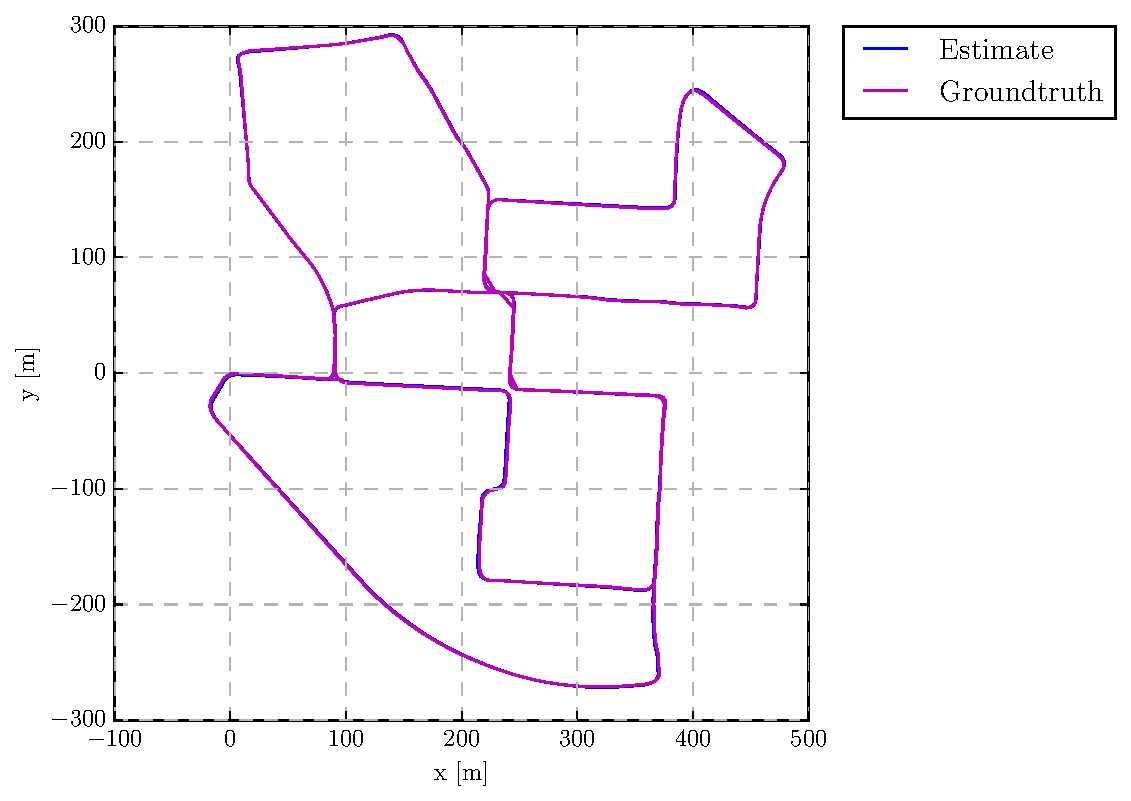
\includegraphics[width=5in]{Chapter4/KITTI/00/gps/plots/trajectory_side_sim3_-1.pdf}
	\caption{Mapping results of the entire sequence without partial sequence.}
	\label{fig:kitticlientmapping} 
\end{figure}

\begin{figure}
	\centering
	\subfigure[Mapping result of Seq.0 compared with ground truth.]{
		\begin{minipage}[t]{0.4\linewidth}
			\centering
			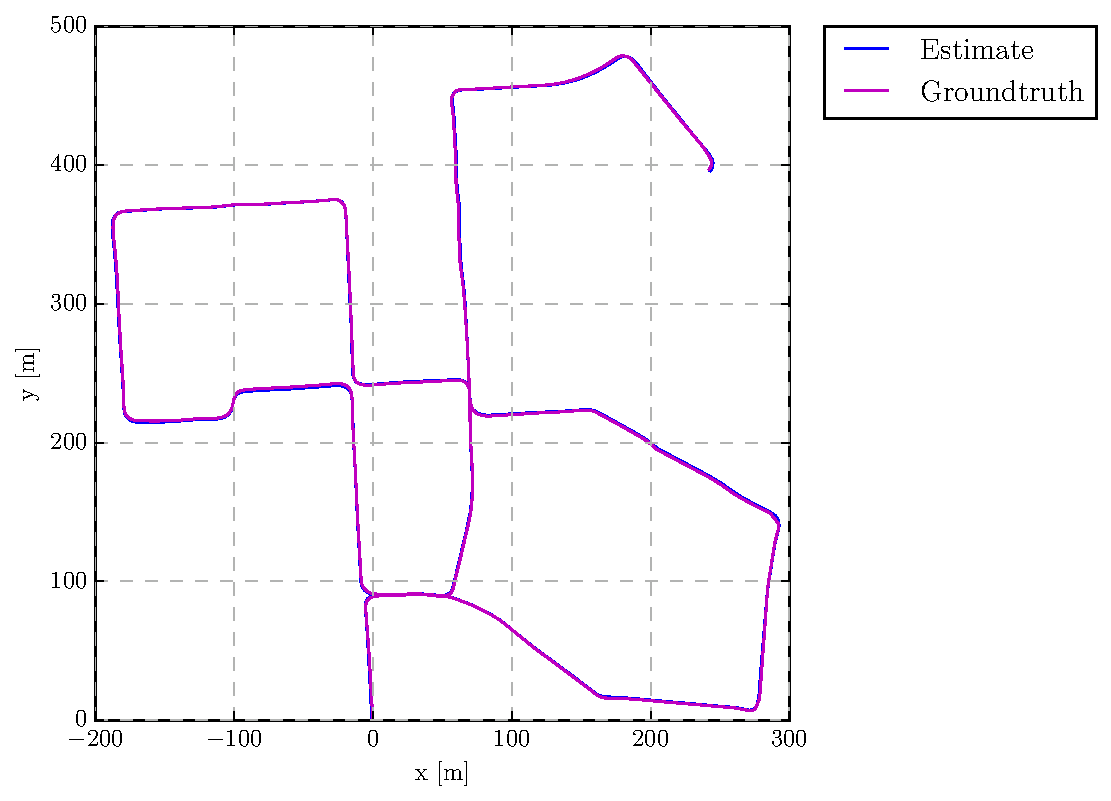
\includegraphics[width=2in]{Chapter4/KITTI/00server/32/plots/trajectory_side_sim3_-1.pdf}
			%\caption{fig1}
		\end{minipage}
	}
	\subfigure[Mapping result of Seq.1 compared with ground truth.]{
		\begin{minipage}[t]{0.4\linewidth}
			\centering
			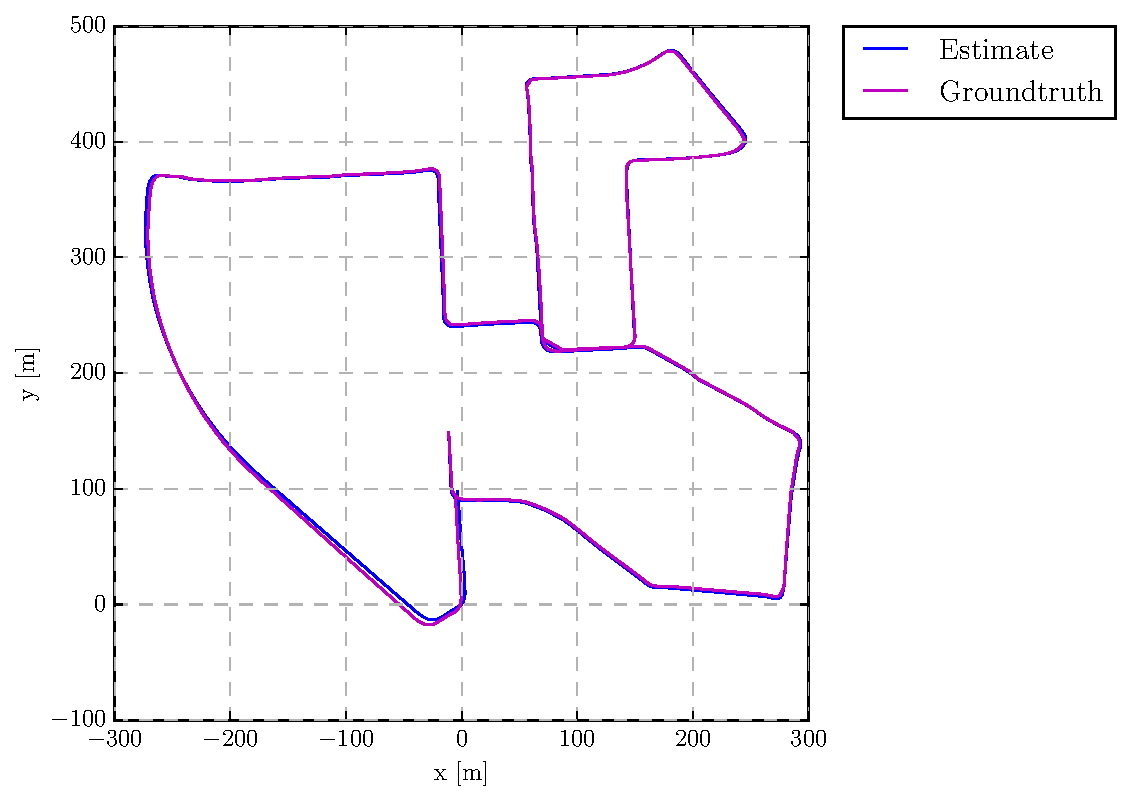
\includegraphics[width=2in]{Chapter4/KITTI/00server/33/plots/trajectory_side_sim3_-1.pdf}
			%\caption{fig2}
		\end{minipage}
	}
	\vfill
	\subfigure[Map Fusion results of Seq.0 and Seq.1 compared with ground truth.]{
		\begin{minipage}[t]{\linewidth}
			\centering
			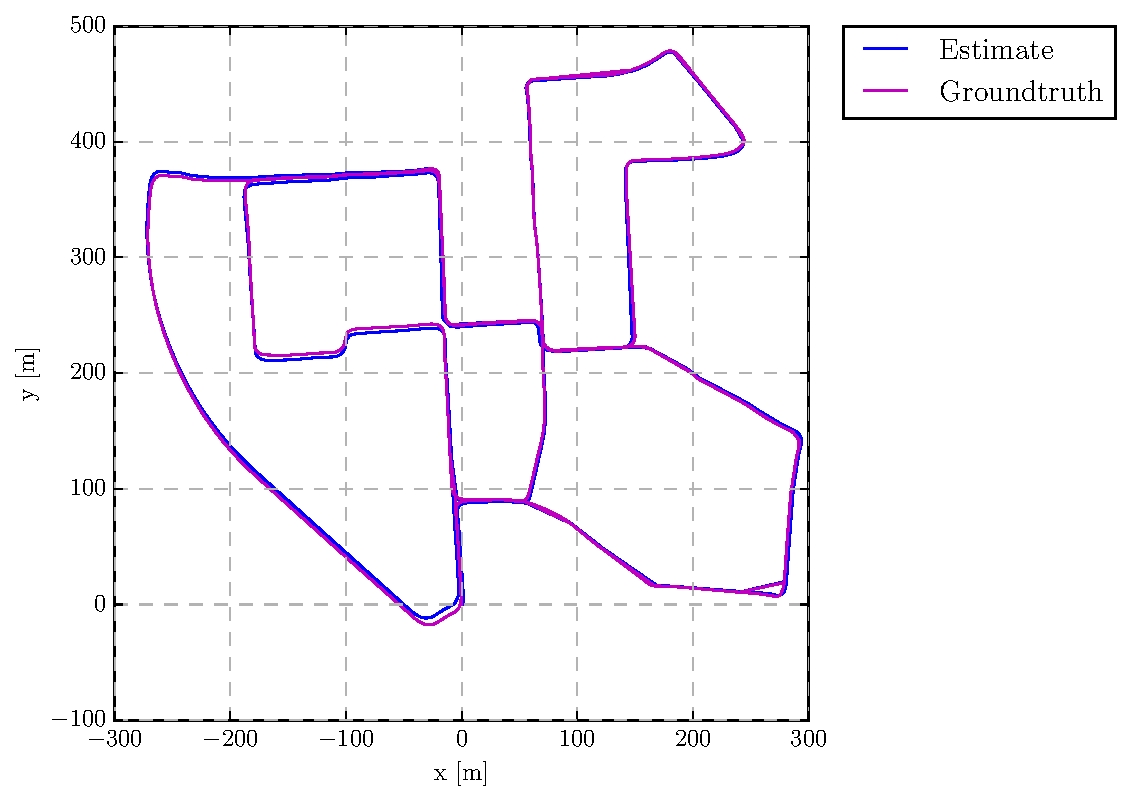
\includegraphics[width=5in]{Chapter4/KITTI/00server/plots/trajectory_side_sim3_-1.pdf}
			%\caption{fig1}
		\end{minipage}
	}
	\caption{Mapping results of Seq.0 and Seq.1, and the map fusion results of KITTI Datasets.}
	\label{fig:kittiresults}
\end{figure}

\begin{figure}
	\centering
	\subfigure[Relative translation error.]{
		\label{sfig:kittireltran}
		\begin{minipage}[t]{0.4\linewidth}
			\centering
			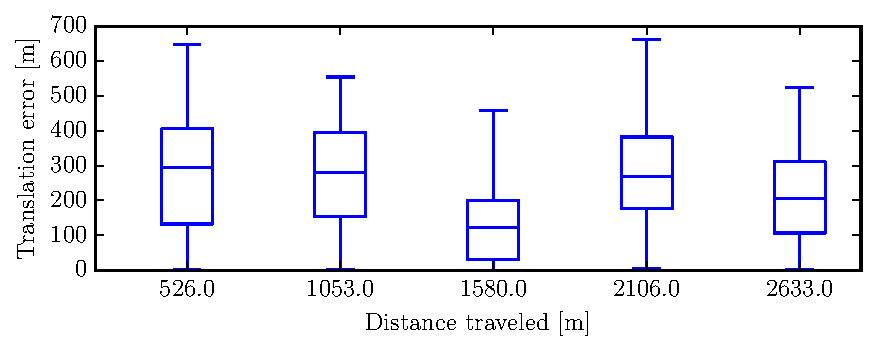
\includegraphics[width=2in]{Chapter4/KITTI/00server/plots/rel_translation_error.pdf}
			%\caption{fig1}
		\end{minipage}
	}
	\subfigure[Relative translation error by percent.]{
		\label{sfig:kittireltranper}
		\begin{minipage}[t]{0.4\linewidth}
			\centering
			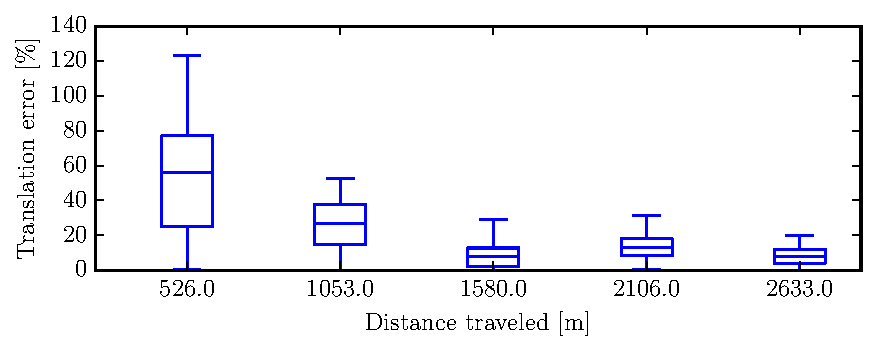
\includegraphics[width=2in]{Chapter4/KITTI/00server/plots/rel_translation_error_perc.pdf}
			%\caption{fig2}
		\end{minipage}
	}
	\vfill
	\subfigure[Relative yaw error.]{
		\label{sfig:kittirelyaw}
		\begin{minipage}[t]{0.4\linewidth}
			\centering
			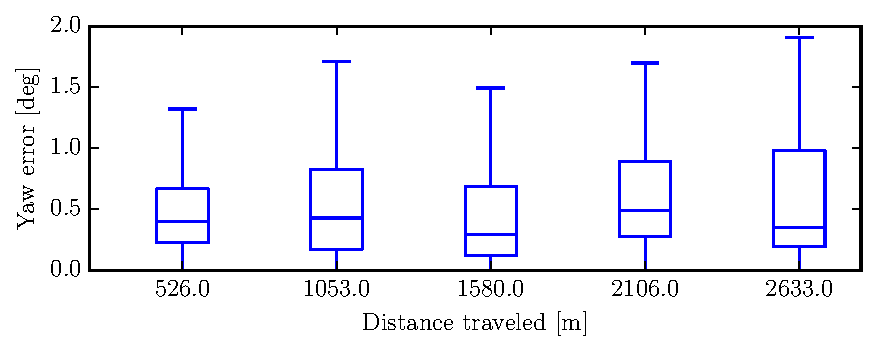
\includegraphics[width=2in]{Chapter4/KITTI/00server/plots/rel_yaw_error.pdf}
			%\caption{fig1}
		\end{minipage}
	}
\ifoutputscaleerror
	\subfigure[Scale error.]{
		\label{sfig:kittiscaleerr}
		\begin{minipage}[t]{0.4\linewidth}
			\centering
			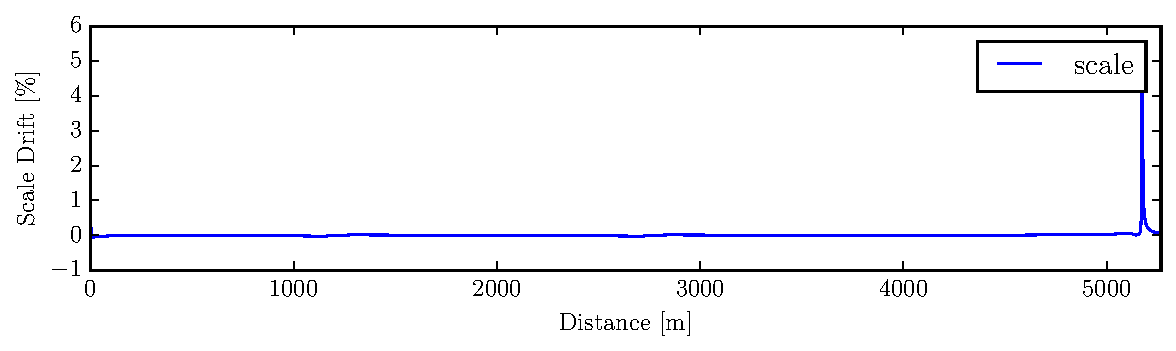
\includegraphics[width=2in]{Chapter4/KITTI/00server/plots/scale_error_sim3_-1.pdf}
			%\caption{fig2}
		\end{minipage}
	}
\fi
	\caption{Quantitative evaluation results of fused map of KITTI Datasets.}
	\label{fig:kittiquanresult}
\end{figure}

\begin{table*}
	\centering
	\caption{Quantitative results of map fusion evaluation on KITTI partial sequences.}
	\begin{threeparttable}
	\ifoutputscaleerror
	\begin{tabular}{|c|c|c|c|c|}
		\hline
		Distance(m)\tnote{1} & Rel. Trans.(m)\tnote{2}  & Rel. Trans.($\%$)\tnote{3} & Rel. Yaw(deg)\tnote{4} & Scale Err.($\%$)\tnote{5}  \\
		\hline
		526& 283.40 & 53.88 & 0.46& - \\
		\hline
		1053&276.16& 26.23 & 0.51 & - \\
		\hline
		1580&153.74& 9.73 & 0.48 & - \\
		\hline
		2106&284.95& 13.53 & 0.57 & - \\
		\hline
		2633&219.66& 8.34 & 0.54 & -0.15\\
		\hline
	\end{tabular}
      \begin{tablenotes}
		\footnotesize
		\item[1] Distance in meter traveled before each time of statistics. 
		\item[2] Mean relative translation error in meter.
		\item[3] Mean relative translation error in percent.
		\item[4] Mean relative yaw error in degree.
		\item[5] Median scale error in percent.
	\end{tablenotes}
\fi

	\begin{tabular}{|c|c|c|c|c|}
	\hline
	Distance(m)\tnote{1} & Rel. Trans.(m)\tnote{2}  & Rel. Trans.($\%$)\tnote{3} & Rel. Yaw(deg)\tnote{4} \\
	\hline
	526& 283.40 & 53.88 & 0.46 \\
	\hline
	1053&276.16& 26.23 & 0.51  \\
	\hline
	1580&153.74& 9.73 & 0.48  \\
	\hline
	2106&284.95& 13.53 & 0.57  \\
	\hline
	2633&219.66& 8.34 & 0.54 \\
	\hline
\end{tabular}
\begin{tablenotes}
	\footnotesize
	\item[1] Distance in meter traveled before each time of statistics. 
	\item[2] Mean relative translation error in meter.
	\item[3] Mean relative translation error in percent.
	\item[4] Mean relative yaw error in degree.
\end{tablenotes}


	\end{threeparttable}
	\label{tbl:kittiquanresult}
\end{table*}

\subsection{NTU Datasets}

An obvious drawback of the evaluation on KITTI dataset is the images which are overlapped by two clients are exactly identical because they are extracted from the same sequence. Therefore, the results are expected to be much better than real-world applications in which case it is impossible the images recorded by different clients can be identical.

In order to get more reliable and convincing evaluation results of  CORB-SLAM system, another evaluation on multi ground robots is performed utilizing NTU Datasets. Bag.0 and Bag.1 described in Section \ref{sec:ntuinfo} are selected in this test. These two bags recorded by two UGVs, have different starting and ending location, with limited overlapping, which is much more similar to the case of real-world applications. Clients' mapping results and map fusion results in the server end compared to ground truth trajectories are demonstrated in Figure \ref{fig:ntubag01serverresults}. And ground truth information is provided in Figure \ref{fig:ntubag01gt} for reference. Quantitative results of the fused global map are represented in Figure \ref{fig:ntuquanresult} and Table \ref{tbl:ntuquanresult}. Quantitative results of each client are provided in Figure \ref{fig:ntubag0quanresult}, \ref{fig:ntubag1quanresult} and Table \ref{tbl:ntubag0quanresult}, \ref{tbl:ntubag1quanresult} in the same format as above.

Results are further discussed in Section \ref{sec:disussmultiground}.

\begin{figure}
	\centering
	\subfigure[Ground truth trajectory of Bag.0.]{
		\begin{minipage}[t]{0.4\linewidth}
			\centering
			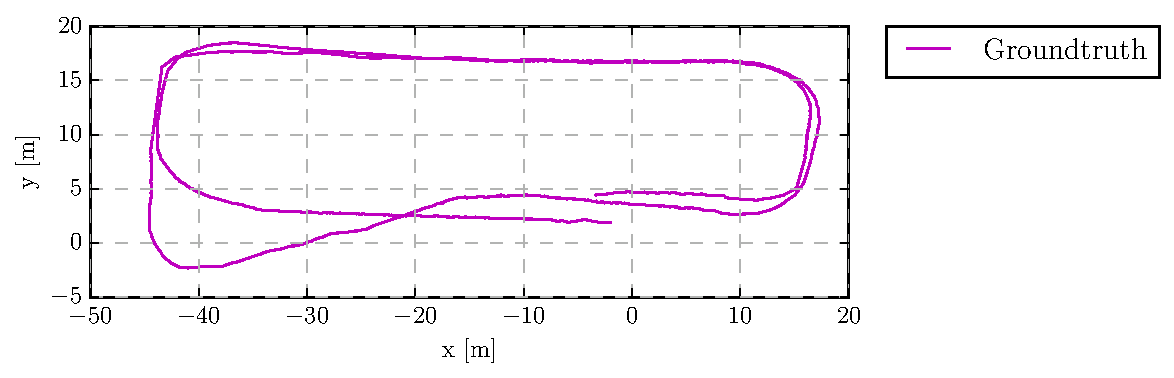
\includegraphics[width=2in]{Chapter4/NTU/0446/plots/trajectory_top_gt_sim3_-1.pdf}
			%\caption{fig1}
		\end{minipage}
	}
	\subfigure[Ground truth trajectory of Bag.1.]{
		\begin{minipage}[t]{0.4\linewidth}
			\centering
			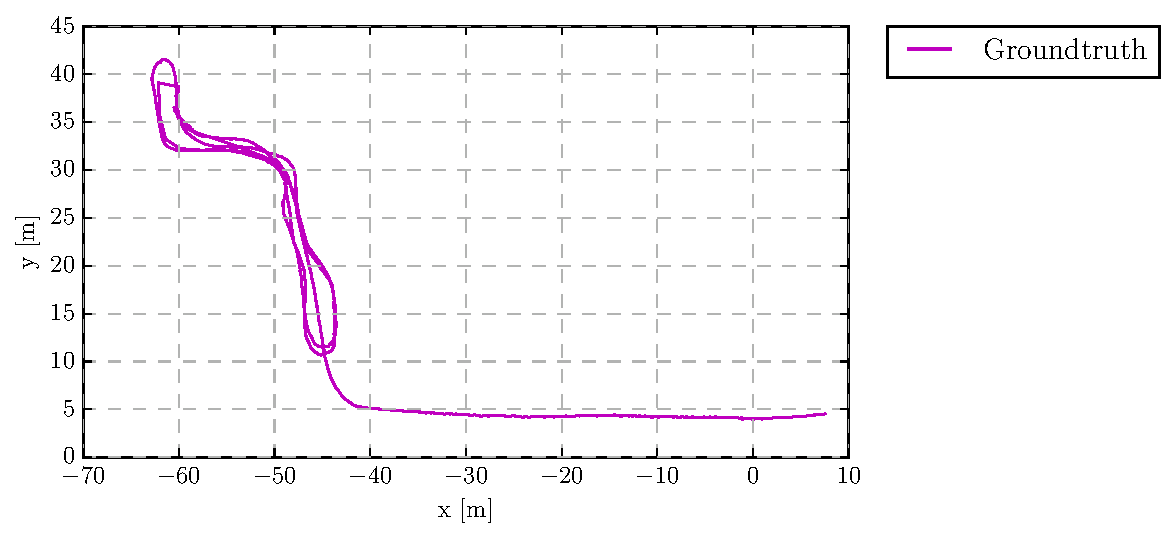
\includegraphics[width=2in]{Chapter4/NTU/0454/plots/trajectory_top_gt_sim3_-1.pdf}
			%\caption{fig2}
		\end{minipage}
	}
	\vfill
	\subfigure[Complete ground truth trajectory of Bag.0 and Bag.1.]{
		\begin{minipage}[t]{\linewidth}
			\centering
			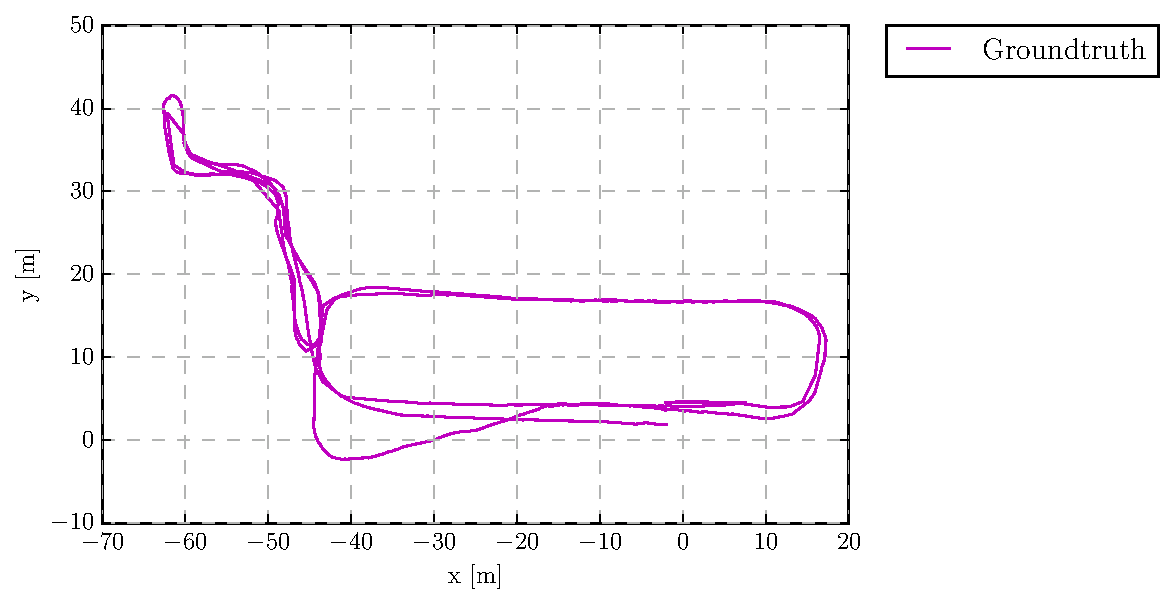
\includegraphics[width=5in]{Chapter4/NTU/server/trajectory_top_gt_sim3_-1.pdf}
			%\caption{fig1}
		\end{minipage}
	}
	\caption{Ground truth trajectory of partial and complete bags of NTU Datasets.}
	\label{fig:ntubag01gt}
\end{figure}

\begin{figure}
	\centering
	\subfigure[Mapping result of Bag.0 compared with ground truth.]{
		\begin{minipage}[t]{0.4\linewidth}
			\centering
			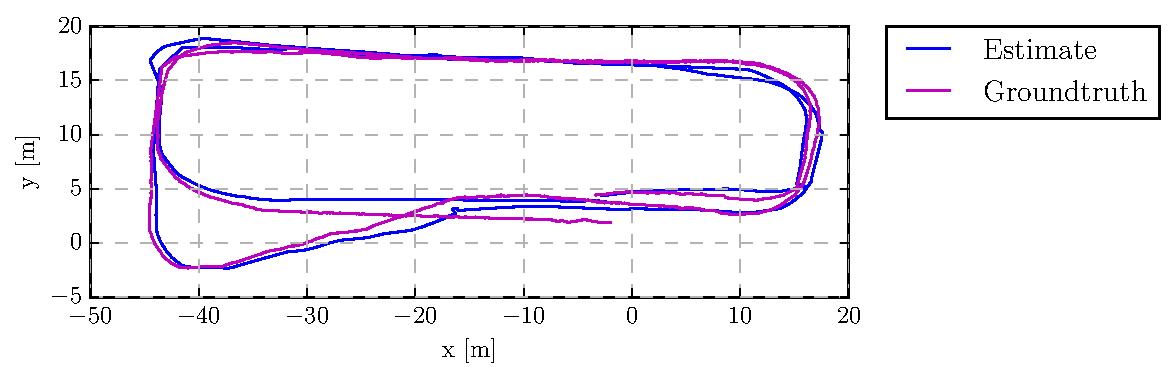
\includegraphics[width=2in]{Chapter4/NTU/0446/plots/trajectory_top_sim3_-1.pdf}
			%\caption{fig1}
		\end{minipage}
	}
	\subfigure[Mapping result of Bag.1 compared with ground truth.]{
		\begin{minipage}[t]{0.4\linewidth}
			\centering
			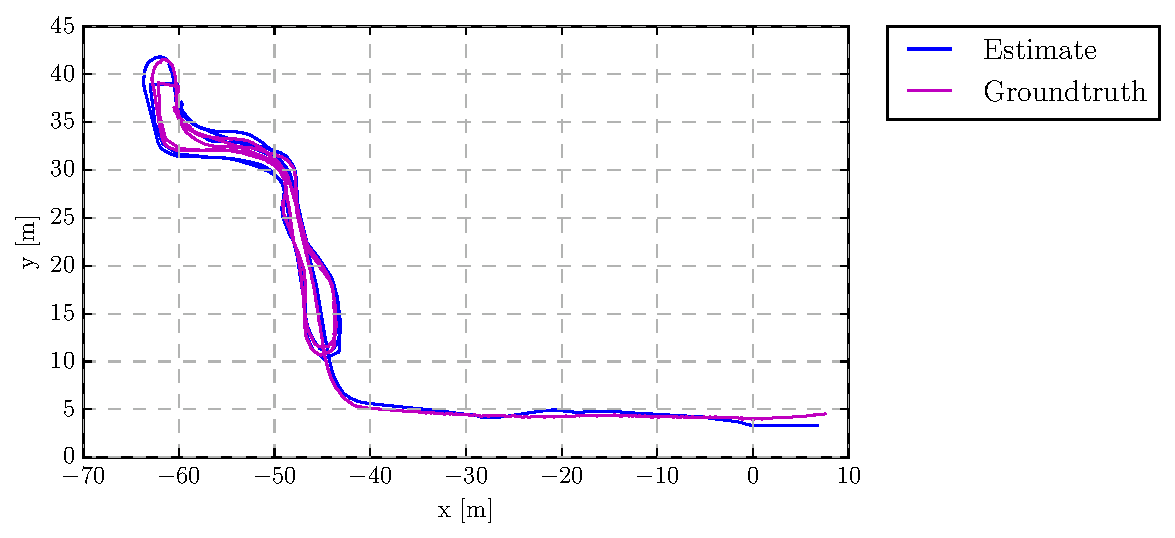
\includegraphics[width=2in]{Chapter4/NTU/0454/plots/trajectory_top_sim3_-1.pdf}
			%\caption{fig2}
		\end{minipage}
	}
	\vfill
	\subfigure[Map Fusion results in server end of Bag.0 and Bag.1.]{
		\begin{minipage}[t]{\linewidth}
			\centering
			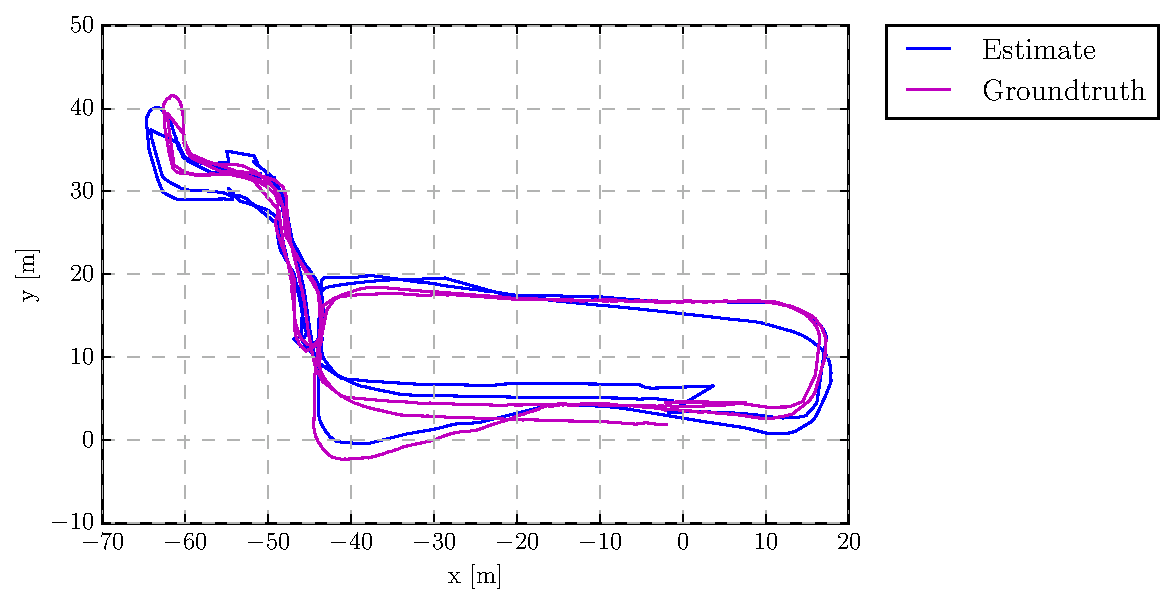
\includegraphics[width=5in]{Chapter4/NTU/server/trajectory_top_sim3_-1.pdf}
			%\caption{fig1}
		\end{minipage}
	}
	\caption{Mapping results of Bag.0 and Bag.1 and the map fusion result of server.}
	\label{fig:ntubag01serverresults}
\end{figure}

\begin{figure}
	\centering
	\subfigure[Relative translation error.]{
		\begin{minipage}[t]{0.4\linewidth}
			\centering
			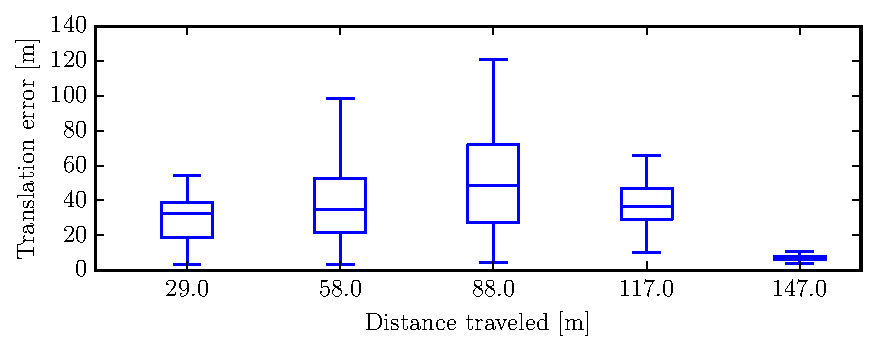
\includegraphics[width=2in]{Chapter4/NTU/0446/plots/rel_translation_error.pdf}
			%\caption{fig1}
		\end{minipage}
	}
	\subfigure[Relative translation error by percent.]{
		\begin{minipage}[t]{0.4\linewidth}
			\centering
			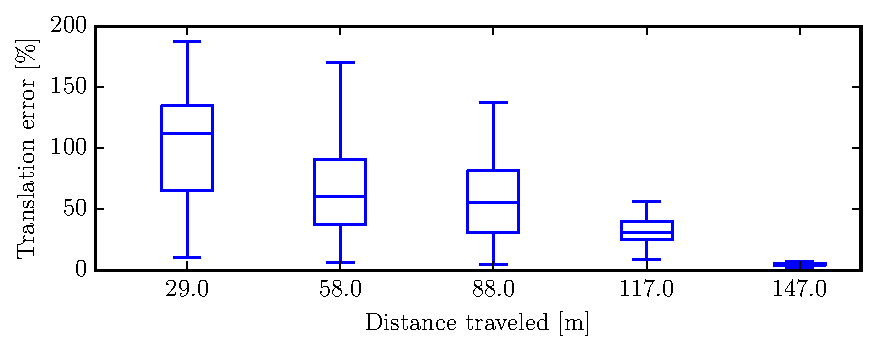
\includegraphics[width=2in]{Chapter4/NTU/0446/plots/rel_translation_error_perc.pdf}
			%\caption{fig2}
		\end{minipage}
	}
	\vfill
	\subfigure[Relative yaw error.]{
		\begin{minipage}[t]{0.4\linewidth}
			\centering
			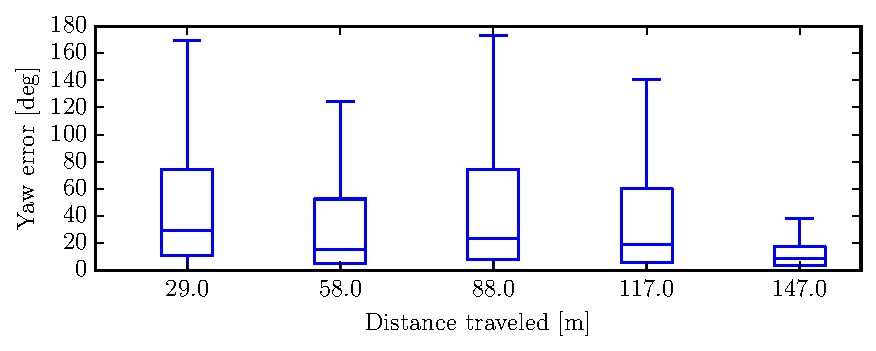
\includegraphics[width=2in]{Chapter4/NTU/0446/plots/rel_yaw_error.pdf}
			%\caption{fig1}
		\end{minipage}
	}
\ifoutputscaleerror
	\subfigure[Scale error.]{
		\begin{minipage}[t]{0.4\linewidth}
			\centering
			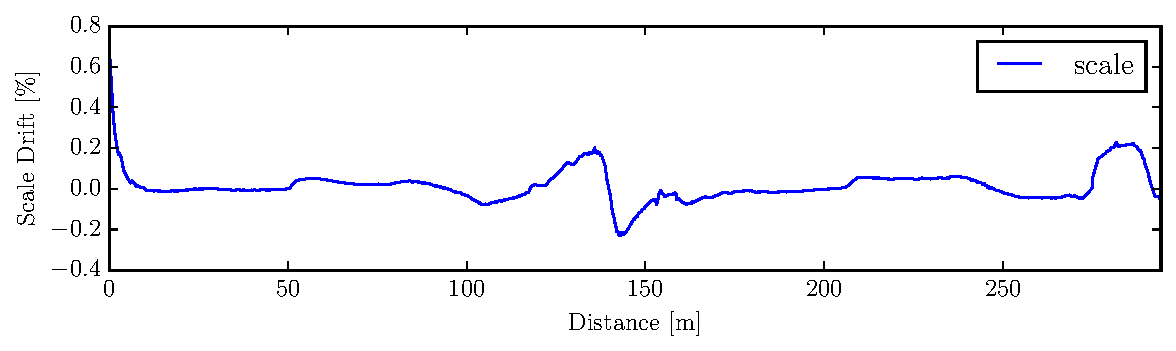
\includegraphics[width=2in]{Chapter4/NTU/0446/plots/scale_error_sim3_-1.pdf}
			%\caption{fig2}
		\end{minipage}
	}
\fi
	\caption{Quantitative evaluation results of mapping Bag.0 of NTU Datasets.}
	\label{fig:ntubag0quanresult}
\end{figure}

\begin{figure}
	\centering
	\subfigure[Relative translation error.]{
		\begin{minipage}[t]{0.4\linewidth}
			\centering
			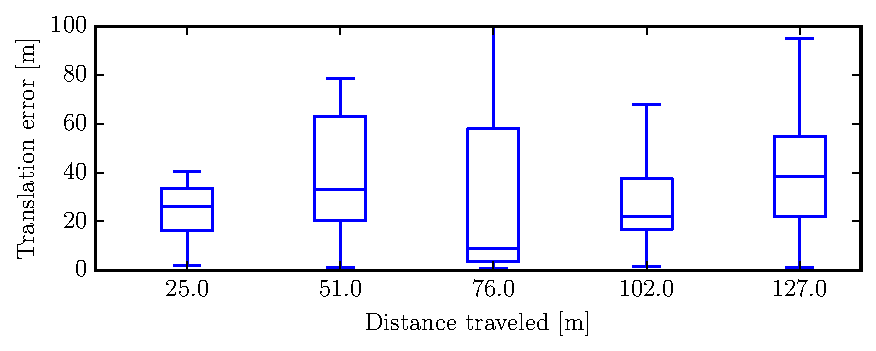
\includegraphics[width=2in]{Chapter4/NTU/0454/plots/rel_translation_error.pdf}
			%\caption{fig1}
		\end{minipage}
	}
	\subfigure[Relative translation error by percent.]{
		\begin{minipage}[t]{0.4\linewidth}
			\centering
			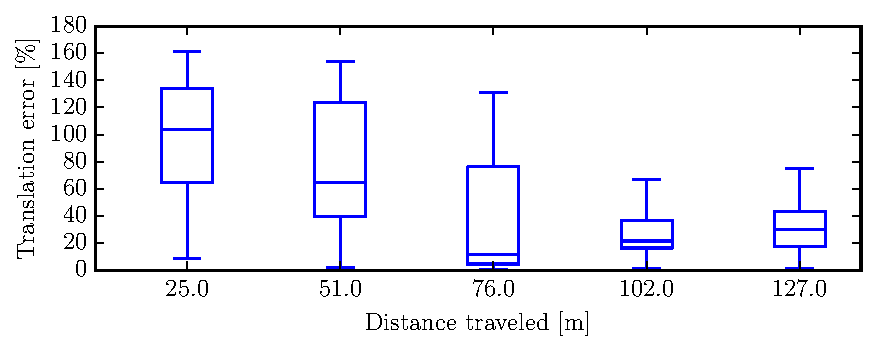
\includegraphics[width=2in]{Chapter4/NTU/0454/plots/rel_translation_error_perc.pdf}
			%\caption{fig2}
		\end{minipage}
	}
	\vfill
	\subfigure[Relative yaw error.]{
		\begin{minipage}[t]{0.4\linewidth}
			\centering
			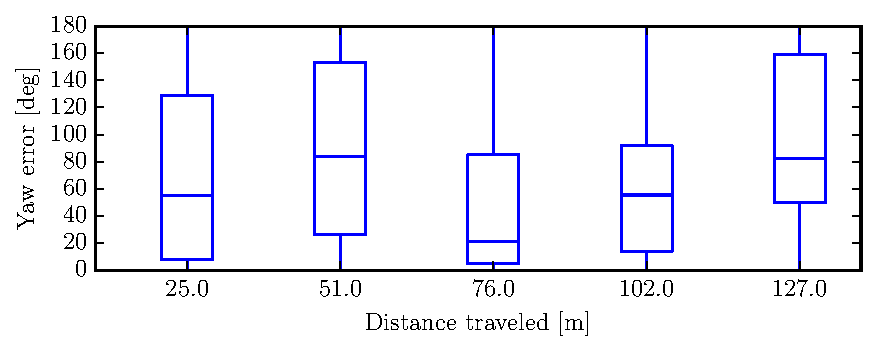
\includegraphics[width=2in]{Chapter4/NTU/0454/plots/rel_yaw_error.pdf}
			%\caption{fig1}
		\end{minipage}
	}
\ifoutputscaleerror
	\subfigure[Scale error.]{
		\begin{minipage}[t]{0.4\linewidth}
			\centering
			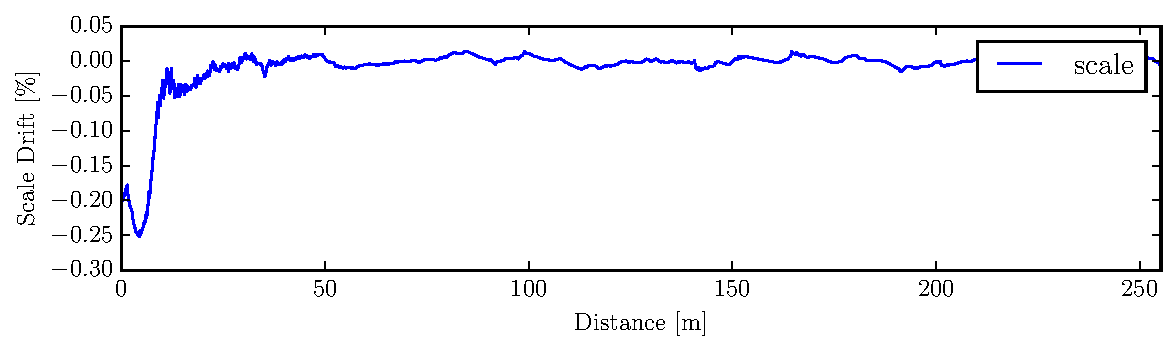
\includegraphics[width=2in]{Chapter4/NTU/0454/plots/scale_error_sim3_-1.pdf}
			%\caption{fig2}
		\end{minipage}
	}
\fi
	\caption{Quantitative evaluation results of mapping Bag.1 of NTU Datasets.}
	\label{fig:ntubag1quanresult}
\end{figure}

\begin{figure}
	\centering
	\subfigure[Relative translation error.]{
		\begin{minipage}[t]{0.4\linewidth}
			\centering
			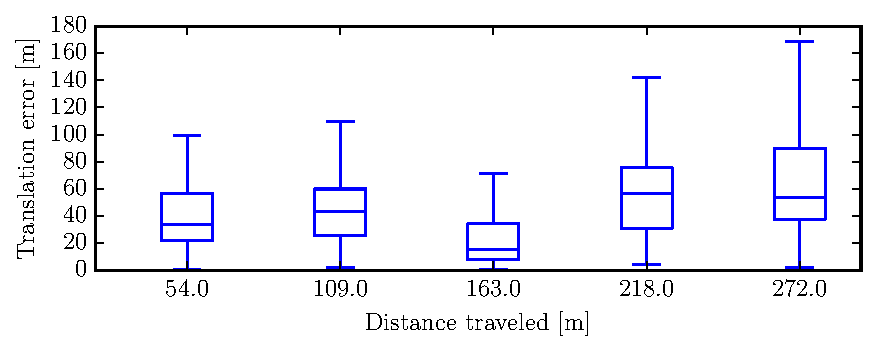
\includegraphics[width=2in]{Chapter4/NTU/server/rel_translation_error.pdf}
			%\caption{fig1}
		\end{minipage}
	}
	\subfigure[Relative translation error by percent.]{
		\begin{minipage}[t]{0.4\linewidth}
			\centering
			\includegraphics[width=2in]{Chapter4/NTU/server/rel_translation_error_perc.pdf}
			%\caption{fig2}
		\end{minipage}
	}
	\vfill
	\subfigure[Relative yaw error.]{
		\begin{minipage}[t]{0.4\linewidth}
			\centering
			\includegraphics[width=2in]{Chapter4/NTU/server/rel_yaw_error.pdf}
			%\caption{fig1}
		\end{minipage}
	}
\ifoutputscaleerror
	\subfigure[Scale error.]{
		\begin{minipage}[t]{0.4\linewidth}
			\centering
			\includegraphics[width=2in]{Chapter4/NTU/server/scale_error_sim3_-1.pdf}
			%\caption{fig2}
		\end{minipage}
	}
\fi
	\caption{Quantitative evaluation results of fused map of NTU Datasets.}
	\label{fig:ntuquanresult}
\end{figure}

\begin{table*}
	\centering
	\caption{Quantitative results of mapping evaluation on Bag.0 NTU Datasets.}
	\begin{threeparttable}
		\begin{tabular}{|c|c|c|c|c|}
			\hline
			Distance(m)\tnote{1} & Rel. Trans.(m)\tnote{2}  & Rel. Trans.($\%$)\tnote{3} & Rel. Yaw(deg)\tnote{4} \\
			\hline
			29& 28.75 & 99.13 & 45.55 \\
			\hline
			58&38.97& 67.19 & 34.89 \\
			\hline
			88&51.96& 59.05 & 43.74  \\
			\hline
			117&37.88&32.38 & 36.31  \\
			\hline
			147&9.29& 6.32 & 10.71 \\
			\hline
		\end{tabular}
		\begin{tablenotes}
			\footnotesize
			\item[1] Distance in meter traveled before each time of statistics. 
			\item[2] Mean relative translation error in meter.
			\item[3] Mean relative translation error in percent.
			\item[4] Mean relative yaw error in degree.
		\end{tablenotes}
	
	\ifoutputscaleerror
			\begin{tabular}{|c|c|c|c|c|}
		\hline
		Distance(m)\tnote{1} & Rel. Trans.(m)\tnote{2}  & Rel. Trans.($\%$)\tnote{3} & Rel. Yaw(deg)\tnote{4} & Scale Err.($\%$)\tnote{5}  \\
		\hline
		29& 28.75 & 99.13 & 45.55& - \\
		\hline
		58&38.97& 67.19 & 34.89 & - \\
		\hline
		88&51.96& 59.05 & 43.74 & - \\
		\hline
		117&37.88&32.38 & 36.31 & - \\
		\hline
		147&9.29& 6.32 & 10.71 & 0.44\\
		\hline
	\end{tabular}
	\begin{tablenotes}
		\footnotesize
		\item[1] Distance in meter traveled before each time of statistics. 
		\item[2] Mean relative translation error in meter.
		\item[3] Mean relative translation error in percent.
		\item[4] Mean relative yaw error in degree.
		\item[5] Median scale error in percent.
	\end{tablenotes}
	\fi

	\end{threeparttable}
	\label{tbl:ntubag0quanresult}
\end{table*}

\begin{table*}
	\centering
	\caption{Quantitative results of mapping evaluation on Bag.1 NTU Datasets.}
	\begin{threeparttable}
		
		\begin{tabular}{|c|c|c|c|c|}
			\hline
			Distance(m)\tnote{1} & Rel. Trans.(m)\tnote{2}  & Rel. Trans.($\%$)\tnote{3} & Rel. Yaw(deg)\tnote{4}   \\
			\hline
			25& 24.79 & 99.17 & 71.03 \\
			\hline
			51&37.20& 72.94 & 88.44  \\
			\hline
			76&29.90& 39.34 & 49.64  \\
			\hline
			102&34.40&33.73& 67.14  \\
			\hline
			127&38.99& 30.70 & 91.89 \\
			\hline
		\end{tabular}
		\begin{tablenotes}
			\footnotesize
			\item[1] Distance in meter traveled before each time of statistics. 
			\item[2] Mean relative translation error in meter.
			\item[3] Mean relative translation error in percent.
			\item[4] Mean relative yaw error in degree.
		\end{tablenotes}
	
	\ifoutputscaleerror
	\begin{tabular}{|c|c|c|c|c|}
		\hline
		Distance(m)\tnote{1} & Rel. Trans.(m)\tnote{2}  & Rel. Trans.($\%$)\tnote{3} & Rel. Yaw(deg)\tnote{4} & Scale Err.($\%$)\tnote{5}  \\
		\hline
		25& 24.79 & 99.17 & 71.03 & - \\
		\hline
		51&37.20& 72.94 & 88.44 & - \\
		\hline
		76&29.90& 39.34 & 49.64 & - \\
		\hline
		102&34.40&33.73& 67.14 & - \\
		\hline
		127&38.99& 30.70 & 91.89 & -1.31\\
		\hline
	\end{tabular}
	\begin{tablenotes}
		\footnotesize
		\item[1] Distance in meter traveled before each time of statistics. 
		\item[2] Mean relative translation error in meter.
		\item[3] Mean relative translation error in percent.
		\item[4] Mean relative yaw error in degree.
		\item[5] Median scale error in percent.
	\end{tablenotes}
\fi
	\end{threeparttable}
	\label{tbl:ntubag1quanresult}
\end{table*}

\begin{table*}
	\centering
	\caption{Quantitative results of map fusion evaluation on  NTU Datasets.}
	\begin{threeparttable}
		\begin{tabular}{|c|c|c|c|c|}
			\hline
			Distance(m)\tnote{1} & Rel. Trans.(m)\tnote{2}  & Rel. Trans.($\%$)\tnote{3} & Rel. Yaw(deg)\tnote{4}  \\
			\hline
			54& 39.38 & 72.93 & 44.39 \\
			\hline
			109&44.88& 41.18 & 57.01  \\
			\hline
			163&26.09& 16.00 & 32.12  \\
			\hline
			218&54.99& 25.23 & 46.11  \\
			\hline
			272&64.66& 23.77 & 54.65 \\
			\hline
		\end{tabular}
		\begin{tablenotes}
			\footnotesize
			\item[1] Distance in meter traveled before each time of statistics. 
			\item[2] Mean relative translation error in meter.
			\item[3] Mean relative translation error in percent.
			\item[4] Mean relative yaw error in degree.
		\end{tablenotes}
	
	\ifoutputscaleerror
			\begin{tabular}{|c|c|c|c|c|}
		\hline
		Distance(m)\tnote{1} & Rel. Trans.(m)\tnote{2}  & Rel. Trans.($\%$)\tnote{3} & Rel. Yaw(deg)\tnote{4} & Scale Err.($\%$)\tnote{5}  \\
		\hline
		54& 39.38 & 72.93 & 44.39& - \\
		\hline
		109&44.88& 41.18 & 57.01 & - \\
		\hline
		163&26.09& 16.00 & 32.12 & - \\
		\hline
		218&54.99& 25.23 & 46.11 & - \\
		\hline
		272&64.66& 23.77 & 54.65 & 0.10\\
		\hline
	\end{tabular}
	\begin{tablenotes}
		\footnotesize
		\item[1] Distance in meter traveled before each time of statistics. 
		\item[2] Mean relative translation error in meter.
		\item[3] Mean relative translation error in percent.
		\item[4] Mean relative yaw error in degree.
		\item[5] Median scale error in percent.
	\end{tablenotes}
\fi
	\end{threeparttable}
	\label{tbl:ntuquanresult}
\end{table*}


%\subsection{Evaluation on multi hybrid robots}
%The evaluation of 

\section{Evaluation under different illumination}
\subsubsection{Oxford RobotCar Datasets}
CORB-SLAM system integrated with illumination variance is firstly evaluated on the selected sequences of Oxford RobotCar Datasets, and then the mapping results are compared with the ground truth trajectories, with quantitative evaluation results calculated.

Two partial sequences are selected according the following principles: 
\begin{enumerate}[1.]
	\item Exclude the overexposed photo, which will cause tracking lost in ORBSLAM system.
	Because the dataset was collected in real-world outdoor street environment, there are some frames with overexposure e.g. Figure \ref{fig:robotcaroverexposed}, which cannot be process by vSLAM. Therefore, in this work, this dataset is intercepted into two sub sequences excluding overexposed images.

	\begin{figure}[H]
		\centering
		\includegraphics[width=5in]{Chapter4/robotcaroverexposed.eps}
		\caption{Image sequence with overexposed frames in RobotCar dataset.}
		\label{fig:robotcaroverexposed} 
	\end{figure}

	\item Avoid partial sequences where traffic congestion occurred. Because RobotCar Datasets are recorded in different hours during daytime, there are congestion starting at approximately 15:00.
	
%\begin{figure}[H]
%	\centering
%	\includegraphics[width=5in]{thereisafigure.eps}
%	\caption{Images when traffic congestion occurred in RobotCar datasets.}
%	\label{fig:robotcarcongestion} 
%\end{figure}

	\item Select partial sequence containing images with overlapping under different illumination conditions and in different season, as shown in Figure \ref{fig:robotcarcomparisonseason}. 
\end{enumerate}

According to the above selection principles, the two sub sequences selected are listed in Table \ref{tbl:robotcarpartial}. The ground truth GPS/INS trajectories of two sub sequences and the combined overall trajectories are shown in Figure \ref{fig:robotcarseq01servergt}. The estimate trajectories and the fused map of two partial sequences are shown in Figure \ref{fig:robotcarseq01serverresults}. Results of Oxford RobotCar Datasets are further discussed in Section \ref{sec:discusslifelong}.

\begin{table*}
	\centering
	\caption{Partial datasets selected in RobotCar dataset.}
	\begin{tabular}{|c|c|c|c|c|}
		\hline
		Seq. No. & Data(M/D/Y) & Time & Weather & Timestamps  \\
		\hline
		0&07/14/2014&14:49&\tabincell{c}{summer\\overcast}& \tabincell{c}{1405349847738682 to\\1405350059147905}\\
		\hline
		1&02/24/2014&12:32&\tabincell{c}{winter\\overcast}& \tabincell{c}{1417794166325288 to\\1417794407042717}\\
		\hline
	\end{tabular}
	\label{tbl:robotcarpartial}
\end{table*}

\begin{figure}
	\centering
	\subfigure[Ground truth trajectory of Seq.0.]{
		\begin{minipage}[t]{0.4\linewidth}
			\centering
			\includegraphics[width=2in]{Chapter3/0714gt.eps}
			%\caption{fig1}
		\end{minipage}
	}
	\subfigure[Ground truth trajectory of Seq.0.]{
		\begin{minipage}[t]{0.4\linewidth}
			\centering
			\includegraphics[width=2in]{Chapter3/0224gt.eps}
			%\caption{fig2}
		\end{minipage}
	}
	\vfill
	\subfigure[Overall ground truth trajectory of Seq.0 and Seq.1.]{
		\begin{minipage}[t]{\linewidth}
			\centering
			\includegraphics[width=5in]{Chapter3/overall_gt_top_.eps}
			%\caption{fig1}
		\end{minipage}
	}
	\caption{Ground truth individual and overall trajectories of Seq.0 and Seq.1 in Oxford RobotCar Datasets.}
	\label{fig:robotcarseq01servergt}
\end{figure}

\begin{figure}
	\centering
	\subfigure[Mapping result of Seq.0.]{
		\begin{minipage}[t]{0.4\linewidth}
			\centering
			\includegraphics[width=2in]{Chapter4/robotcar/0714/gps/plots/trajectory_top_sim3_-1.eps}
			%\caption{fig1}
		\end{minipage}
	}
	\subfigure[Mapping result of Seq.1.]{
		\begin{minipage}[t]{0.4\linewidth}
			\centering
			\includegraphics[width=2in]{Chapter4/robotcar/0224/gps/plots/trajectory_top_sim3_-1.eps}
			%\caption{fig2}
		\end{minipage}
	}
	\vfill
	\subfigure[Map Fusion results in server end of Seq.0 and Seq.1.]{
		\begin{minipage}[t]{\linewidth}
			\centering
			\includegraphics[width=5in]{Chapter4/robotcar/plots/trajectory_top_sim3_-1.eps}
			%\caption{fig1}
		\end{minipage}
	}
	\caption{Mapping results of Seq.0 and Seq.1 and the map fusion result of server in Oxford RobotCar Datasets.}
	\label{fig:robotcarseq01serverresults}
\end{figure}

\begin{figure}[H]
	\centering
	\includegraphics[width=5in]{Chapter4/robotcar/plots/trajectory_top_est_sim3_-1.pdf}
	\caption{Map fusion results of Seq.0 and Seq.1 without ground truth in Oxford RobotCar Datasets.}
	\label{fig:robotcarmfresult} 
\end{figure}



%=== END OF CHAPTER FOUR ===
\newpage
